% ******************************* PhD Thesis Template **************************
% Please have a look at the README.md file for info on how to use the template

\documentclass[a4paper,12pt,times,numbered,print,index]{Classes/PhDThesisPSnPDF}

% ******************************************************************************
% ******************************* Class Options ********************************
% *********************** See README for more details **************************
% ******************************************************************************

% `a4paper'(The University of Cambridge PhD thesis guidelines recommends a page
% size a4 - default option) or `a5paper': A5 Paper size is also allowed as per
% the Cambridge University Engineering Deparment guidelines for PhD thesis
%
% `11pt' or `12pt'(default): Font Size 10pt is NOT recommended by the University
% guidelines
%
% `oneside' or `twoside'(default): Printing double side (twoside) or single
% side.
%
% `print': Use `print' for print version with appropriate margins and page
% layout. Leaving the options field blank will activate Online version.
%
% `index': For index at the end of the thesis
%
% `draft': For draft mode without loading any images (same as draft in book)
%
% `abstract': To generate only the title page and abstract page with
% dissertation title and name, to submit to the Student Registry
%
% `chapter`: This option enables only the specified chapter and it's references
%  Useful for review and corrections.
%
% ************************* Custom Page Margins ********************************
%
% `custommargin`: Use `custommargin' in options to activate custom page margins,
% which can be defined in the preamble.tex. Custom margin will override
% print/online margin setup.
%
% *********************** Choosing the Fonts in Class Options ******************
%
% `times' : Times font with math support. (The Cambridge University guidelines
% recommend using times)
%
% `fourier': Utopia Font with Fourier Math font (Font has to be installed) 
%            It's a free font.
%
% `customfont': Use `customfont' option in the document class and load the
% package in the preamble.tex
%
% default or leave empty: `Latin Modern' font will be loaded.
%
% ********************** Choosing the Bibliography style ***********************
%
% `authoryear': For author-year citation eg., Krishna (2013)
%
% `numbered': (Default Option) For numbered and sorted citation e.g., [1,5,2]
%
% `custombib': Define your own bibliography style in the `preamble.tex' file.
%              `\RequirePackage[square, sort, numbers, authoryear]{natbib}'. 
%              This can be also used to load biblatex instead of natbib 
%              (See Preamble) 
%
% **************************** Choosing the Page Style *************************
%
% `default (leave empty)': For Page Numbers in Header (Left Even, Right Odd) and
% Chapter Name in Header (Right Even) and Section Name (Left Odd). Blank Footer.
%
% `PageStyleI': Chapter Name next & Page Number on Even Side (Left Even).
% Section Name & Page Number in Header on Odd Side (Right Odd). Footer is empty.
%
% `PageStyleII': Chapter Name on Even Side (Left Even) in Header. Section Number
% and Section Name in Header on Odd Side (Right Odd). Page numbering in footer


% ********************************** Preamble **********************************
% Preamble: Contains packages and user-defined commands and settings
% ******************************************************************************
% ****************************** Custom Margin *********************************

% Add `custommargin' in the document class options to use this section
% Set {innerside margin / outerside margin / topmargin / bottom margin}  and
% other page dimensions

\ifsetMargin
\else
    \RequirePackage[left=37mm,right=30mm,top=35mm,bottom=30mm]{geometry}
    \setFancyHdr % To apply fancy header after geometry package is loaded
\fi

% *****************************************************************************
% ******************* Fonts (like different typewriter fonts etc.)*************

% Add `customfont' in the document class option to use this section

\ifsetFont
\else
    % Set your custom font here and use `customfont' in options. Leave empty to
    % load computer modern font (default LaTeX font).  

    \RequirePackage{libertine} 
\fi

% *****************************************************************************
% *************************** Bibliography  and References ********************

%\usepackage{cleveref} %Referencing without need to explicitly state fig /table

% Add `custombib' in the document class option to use this section
\ifsetBib % True, Bibliography option is chosen in class options
\else % If custom bibliography style chosen then load bibstyle here

   \RequirePackage[square, sort, numbers, authoryear]{natbib} % CustomBib

% If you would like to use biblatex for your reference management, as opposed to the default `natbibpackage` pass the option `custombib` in the document class. Comment out the previous line to make sure you don't load the natbib package. Uncomment the following lines and specify the location of references.bib file

% \RequirePackage[backend=biber, style=numeric-comp, citestyle=numeric, sorting=nty, natbib=true]{biblatex}
% \bibliography{References/references} %Location of references.bib only for biblatex

\fi


% changes the default name `Bibliography` -> `References'
\renewcommand{\bibname}{References}


% *****************************************************************************
% *************** Changing the Visual Style of Chapter Headings ***************
% Uncomment the section below. Requires titlesec package.

%\RequirePackage{titlesec}
%\newcommand{\PreContentTitleFormat}{\titleformat{\chapter}[display]{\scshape\Large}
%{\Large\filleft{\chaptertitlename} \Huge\thechapter}
%{1ex}{}
%[\vspace{1ex}\titlerule]}
%\newcommand{\ContentTitleFormat}{\titleformat{\chapter}[display]{\scshape\huge}
%{\Large\filleft{\chaptertitlename} \Huge\thechapter}{1ex}
%{\titlerule\vspace{1ex}\filright}
%[\vspace{1ex}\titlerule]}
%\newcommand{\PostContentTitleFormat}{\PreContentTitleFormat}
%\PreContentTitleFormat


% *****************************************************************************
% **************************** Custom Packages ********************************
% *****************************************************************************


% ************************* Algorithms and Pseudocode **************************

%\usepackage{algpseudocode} 


% ********************Captions and Hyperreferencing / URL **********************

% Captions: This makes captions of figures use a boldfaced small font. 
%\RequirePackage[small,bf]{caption}

\RequirePackage[labelsep=space,tableposition=top]{caption} 
\renewcommand{\figurename}{Fig.} %to support older versions of captions.sty

% ************************ Formatting / Footnote *******************************

%\usepackage[perpage]{footmisc} %Range of footnote options 


% ****************************** Line Numbers **********************************

%\RequirePackage{lineno}
%\linenumbers

% ************************** Graphics and figures *****************************

%\usepackage{rotating}
%\usepackage{wrapfig}
%\usepackage{float}
\usepackage{subfig} %note: subfig must be included after the `caption` package. 

% ********************************* Timing Tikz Pictures **************************************
%\usepackage{tikz}
%\usepackage{Packages/svn-prov/svn-prov}
%\usepackage{Packages/tikz-timing/tikz-timing}
%\usepackage{Packages/tikz-timing/tikz-timing-counters}

% -----  works at home , uncomment at home --------
%installed in texlive2013
\usepackage{tikz}
\usepackage{tikz-timing}
%------------------------------------

\usetikzlibrary{arrows,snakes,backgrounds,patterns,matrix,shapes,fit,calc,shadows,plotmarks}
\usetikztiminglibrary[new={char=Q,reset char=R}]{counters}


%\setlength{\PreviewBorder}{5mm}


% ********************************* Table **************************************

%\usepackage{longtable}
%\usepackage{multicol}
%\usepackage{multirow}
%\usepackage{tabularx}

% ********************************* Algorithm **************************************

\usepackage{algorithm}
\usepackage{algorithmic}

% ********************************* Code Listing **************************************

%\usepackage{listings}


% ***************************** Math and SI Units ******************************

\usepackage{amsfonts}
\usepackage{amsmath}
\usepackage{amssymb}
%\usepackage{siunitx} % use this package module for SI units
% ***************************** Usefull Boxes ******************************

\usepackage{fancybox}
\usepackage{latexsym}
\usepackage{stmaryrd}





% ******************************************************************************
% ************************* User Defined Commands ******************************
% ******************************************************************************

% *********** To change the name of Table of Contents / LOF and LOT ************

%\renewcommand{\contentsname}{My Table of Contents}
%\renewcommand{\listfigurename}{My List of Figures}
%\renewcommand{\listtablename}{My List of Tables}


% ********************** TOC depth and numbering depth *************************

\setcounter{secnumdepth}{2}
\setcounter{tocdepth}{2}

% ******************************* Nomenclature *********************************

% To change the name of the Nomenclature section, uncomment the following line

%\renewcommand{\nomname}{Symbols}


% ********************************* Appendix ***********************************

% The default value of both \appendixtocname and \appendixpagename is `Appendices'. These names can all be changed via: 

%\renewcommand{\appendixtocname}{List of appendices}
%\renewcommand{\appendixname}{Appndx}






% ************************ Thesis Information & Meta-data **********************
% Thesis title and author information, refernce file for biblatex
% ************************ Thesis Information & Meta-data **********************
%% The title of the thesis
\title{Hardware Implementation of an Invariant Observer} 
%\texorpdfstring is used for PDF metadata. Usage:
%\texorpdfstring{LaTeX_Version}{PDF Version (non-latex)} eg.,
%\texorpdfstring{$sigma$}{sigma}

%% The full name of the author
\author{Marko Stanisic}

%% Department (eg. Department of Engineering, Maths, Physics)
\dept{Department of Informatics}

%% University and Crest
\university{Technical University of Vienna}
\crest{
\includegraphics[width=0.25\textwidth]{UnivLogo}}

%% You can redefine the submission text:
% Default as per the University guidelines: This thesis is submitted for
% the degree of Doctor of Philosophy
%\renewcommand{\submissiontext}{change the default text here if needed}

%% Full title of the Degree 
\degree{Bachelor of Science}
 
%% College affiliation (optional)
\college{}

%% Submission date
\degreedate{2014} 

%% Meta information
\subject{LaTeX} \keywords{{Invariant Observer} {Bachelor Thesis} {Informatics} {Technical University 
of Vienna}}



% ***************************** Abstract Separate ****************************** 
% To printout only the titlepage and the abstract with the PhD title and the 
% author name for submission to the Student Registry, use the `abstract' option in
% the document class. 

\ifdefineAbstract
 \pagestyle{empty}
 \includeonly{Declaration/declaration, Abstract/abstract} 
\fi

% ***************************** Chapter Mode ***********************************
% The chapter mode allows user to only print particular chapters with references
% Title, Contents, Frontmatter are disabled by default
% Useful option to review a particular chapter or to send it to supervisior.
% To use choose `chapter' option in the document class

\ifdefineChapter
 \includeonly{Chapter3/chapter3} 
\fi

% ******************************** Front Matter ********************************
\begin{document}

\frontmatter

\begin{titlepage}

\maketitle

\end{titlepage}

%% ******************************* Thesis Dedidcation ********************************

\begin{dedication} 

I would like to dedicate this thesis to my loving parents ...

\end{dedication}


% ******************************* Thesis Declaration ********************************

\begin{declaration}

I hereby declare that except where specific reference is made to the work of others, the contents of this dissertation are original and have not been submitted in whole or in part for consideration for any other degree or qualification in this, or any other University. This dissertation is the result of my own work and includes nothing which is the outcome of work done in collaboration, except where specifically indicated in the text. This dissertation contains less than 65,000 words including appendices, bibliography, footnotes, tables and equations and has less than 150 figures.

% Author and date will be inserted automatically from thesis.tex \author \degreedate

\end{declaration}


%% ************************** Thesis Acknowledgements *****************************

\begin{acknowledgements}      


And I would like to acknowledge ...


\end{acknowledgements}

% ************************** Thesis Abstract *****************************
% Use `abstract' as an option in the document class to print only the titlepage and the abstract.
\begin{abstract}
The invariant observer is an approach to implement an alternative hardware realization of the invariant operation
published in the paper \textbf{Runtime Verification of Embedded Real Time Systems.}
The invariant observer monitors at every clock cycle a signal $\phi$ from a Runtime Verification Unit and 
determines whether the signal is in an active state in the last $\tau$ clock cycles.
\end{abstract}


% *********************** Adding TOC and List of Figures ***********************

\tableofcontents

\listoffigures

\listoftables 

% \printnomenclature[space] space can be set as 2.5cm between symbol and
% description
\printnomencl

% ******************************** Main Matter *********************************
\mainmatter

%*****************************************************************************************
%*********************************** First Chapter ***************************************
%*****************************************************************************************

%% Title with Math \texorpdfstring{$\sigma$}{[sigma]} => Title with Math σ

%%A {\em \LaTeX{} class file}\index{\LaTeX{} class file@LaTeX class file} is a file, which holds style information for a particular \LaTeX{}.

%%\begin{eqnarray}
%%CIF: \hspace*{5mm}F_0^j(a) &=& \frac{1}{2\pi \iota} \oint_{\gamma} \frac{F_0^j(z)}{z - a} dz
%%\end{eqnarray}

% reference to a chapter: (see Section~\ref{section1.3})

%formula:	$E^2 = (m_0c^2)^2 + (pc)^2$


\chapter{Introduction}  %Title of the First Chapter

\ifpdf
    \graphicspath{{Chapter1/Figs/Raster/}{Chapter1/Figs/PDF/}{Chapter1/Figs/}}
\else
    \graphicspath{{Chapter1/Figs/Vector/}{Chapter1/Figs/}}
\fi


%********************************** %First Section  **************************************
\section{Overview of the Bachelor Thesis } %Section - 1.1 

In embedded real time systems it is necessary to make efforts to verify a system design.
A system design can be formalized by a mathematical specification for a dynamic system model.
One approach to system design verification is the deduction, that shows that the design implies the requirements. 

In critical Real Time Systems (RTS) timing constraints have to be considered in the requirement engineering.
Such Real Time Systems are modelled by states changing over time.
Time constraints can be formulated as constraints on the duration of critical states. 
A real time logic should be able to specify that real time constraints. Generally it seems that two main classes
of real time logic are present, explicit or implicit temporal logic.\cite{210306} 

Explicit temporal logic is an expression of a time variable. The time variable can be the representation of a time interval or a variable in temporal logic. 
Implicit temporal logic (for example MTL - Metric Temporal Logic) is using temporal operators that constrain the extend of a state.
It is based on interval temporal logic and the duration concept.
Implicit temporal logic can be very useful to express before/after relations between concurrent actions.
For further details \cite{210306} can be a good source of information.
In runtime verification a monitor evaluates executions of a \textbf{System under Test (SUT)} \cite{RTFMBJ13}. 
The evaluation is formalised from a formal specification described in temporal logic.\newpage
For ultra critical systems it is important to meet four major requirements:
\begin{enumerate}
 \item Functionality : cannot change target's behaviour
 \item Certifiability: must avoid re-certification
 \item Timing :	  must not interfere with the target's timing
 \item Swap :     must not exhaust size, weight and power tolerance
\end{enumerate}

A \textbf{Runtime Verification Unit (RVU)} is a verification monitor that meets that four major requirements.
As part of this requirements, the RVU must be separated from SUT.
In fact it is a synthesized hardware that monitors the execution of a SUT.\newline
The topic of my thesis ``Hardware implementation of an Invariant Observer'' can also be considered as a RVU, 
it evaluates the execution of a SUT and checks it for invariance conditions.
My observer is an alternative  implementation of the invariant observer INVARIANT-SYMBOL published in \cite{RTFMBJ13},
that bypass the problem of resource limitation and make use of the significant advantages of a high parallel
\textbf{Field Programmable Gate Array(FPGA)} hardware implementation.
The most important difference is that my observer is not bounded to a specific $\tau$, but the observer in \cite{RTFMBJ13}
are bounded.This feature will be explained in the next section.

In the publication ``\textbf{Real-Time Runtime Verification on Chip} '' \cite{RTFMBJ13} the concept of a RVU and 
the principles of that Verification Framework are described in great detail.\newline\newline
A survey about the functionality of the invariant observer in the following sections.




% \nomenclature[z-cif]{$CIF$}{Cauchy's Integral Formula}                                % first letter Z is for Acronyms 
% \nomenclature[a-F]{$F$}{complex function}                                                   % first letter A is for Roman symbols
% \nomenclature[g-p]{$\pi$}{ $\simeq 3.14\ldots$}                                             % first letter G is for Greek Symbols
% \nomenclature[g-i]{$\iota$}{unit imaginary number $\sqrt{-1}$}                      % first letter G is for Greek Symbols
% \nomenclature[g-g]{$\gamma$}{a simply closed curve on a complex plane}  % first letter G is for Greek Symbols
% \nomenclature[x-i]{$\oint_\gamma$}{integration around a curve $\gamma$} % first letter X is for Other Symbols
% \nomenclature[r-j]{$j$}{superscript index}                                                       % first letter R is for superscripts
% \nomenclature[s-0]{$0$}{subscript index}                                                        % first letter S is for subscripts




%********************************** %Second Section  *************************************
\newpage
\section{The Invariant Observer } %Section - 1.2
This section is a survey about the invariant observer and how it works.
More details about the observers algorithm are presented in the next chapter. \newline
The Invariant Observer acts like the temporal (invariant previously) operator $\boxbox_\tau \phi$
of the Metric Temporal Logic (MTL) and is of course restricted on the past time (ptMTL).
The temporal operator takes an input $\phi$ , the calculation of a propositional
formula, and evaluates if $\phi$ holds for the past $\tau$ execution times , including
the current execution time in a discrete time setting.
For example the logical consequence $e^n \models \boxbox_3 \phi$ expresses that
the current execution $e^n$ (with n as the discrete execution time, n$\in\mathbb{N}$)
is true iff (if and only if) the evaluation of $\phi$ is true now and was also true the last 
$\tau=3$ execution times. In fact the $\boxbox_\tau \phi$ is a specialization of the 
$\boxdot_{[0,\tau]}\phi$ ptMTL operator which inidcates the range of the invariance qualification.\newline
Figure~\ref{fig:inv_example} and Figure~\ref{fig:inv_example_2} show an example for such a temporal operator.
 \newline
%\newpage
\begin{figure}[h] 
\centering 
\begin{tikztimingtable}[scale=1.75,timing/counter/new={char=Q,reset char=R}]
  $n$ & 25{Q} \\
  $e^n \models \phi$ & 1{L}1H2L2H3L3H4L4HL4H\\
  $e^n \models \boxbox_\tau \phi$ & 19{L}1{H}4{L}1{H} \\
  \extracode
  \begin{pgfonlayer}{background}
  \end{pgfonlayer}
  \begin{background}[shift={(0.1,0)},dashed,help lines]
   \vertlines{}
  \end{background}
\end{tikztimingtable}
\caption[Invariant Observer with $\tau=3$]{Example for Invariant Operator  $\boxbox_\tau \phi$  with  $\tau$=3 }
\label{fig:inv_example}
\end{figure}
\newline
\begin{figure}[h] 
\centering 
\begin{tikztimingtable}[scale=1.75,timing/counter/new={char=Q,reset char=R}]
  $n$ & 25{Q} \\
  $e^n \models \phi$ & 1{L}1H2L2H3L3H4L4HL4H\\
  $e^n \models \boxbox_\tau \phi$ & 11{L}1{H}7{L}1{H}4{L}1{H} \\
  \extracode
  \begin{pgfonlayer}{background}
  \end{pgfonlayer}
  \begin{background}[shift={(0.1,0)},dashed,help lines]
   \vertlines{}
  \end{background}
\end{tikztimingtable}
\caption[Invariant Observer with $\tau=2$]{Example for Invariant Operator  $\boxbox_\tau \phi$  with  $\tau$=2 }
\label{fig:inv_example_2}
\end{figure}

My approach of the invariant observer is based on some certain requirements.
The following subsection will discuss these requirements.
 %******************* Subsection 1*******************
\subsection{First Requirement}
To introduce the first requirement we begin with the discussion of the  problem that the calculation
of a atomic propositional formula $\phi$ could take several clock cycles (execution times).
This means that a observer has to wait until the calculation of the proposition is finished.
In \cite{RTFMBJ13} the observer needs to guarantee that it finishes evaluation of atomic propositions
within a tight time bound.
In our case ,if we start calculation of a propositional formula $\phi$ at every clock cycle and the 
calculation itself needs $y$ clock cycles , than we need $y$ observer stages to cover at every clock cycle
a finished calculation. These observer stages are part of the whole observer.
After $y$ clock cycles , at every following clock cycle a calculation of $\phi$ will be available. At least
one observer stage is ready to evaluate a calculation $\phi$ at any time.
In other words, we are implementing temporal pipeline stages that represents components of the
invariant operator and these components together are evaluating the invariance qualification of the proposition $\phi$.
We don't have one observer, in fact the observer is composed from several observer stages.
As a matter of fact, different many clock cycles for the calculation of $\phi$ are possible.
Propositional formulas can be composed from several other complex propositional subformulas.
In some cases a subformula is waiting for the resolution of an another subformula.
In \cite{RTFMBJ13}  this balance is achieved with the restriction of the atomic proposition class
by the abstract domain of logahedron.

%********************************** % Third Section  *************************************
\section{Where does it come from?}  %Section - 1.3 
\label{section1.3}


%*****************************************************************************************
%*********************************** Second Chapter **************************************
%*****************************************************************************************

\chapter{Software Implementation and Algorithm}
\label{chapter:2}
%\ifpdf
%    \graphicspath{{Chapter2/Figs/Raster/}{Chapter2/Figs/PDF/}{Chapter2/Figs/}}
%\else
%    \graphicspath{{Chapter2/Figs/Vector/}{Chapter2/Figs/}}
%\fi


\section{Algorithm of the Invariant Observer Stages}
\label{chapter:sub:1}
The following algorithm shows the proper behaviour of an observer stage.\newline

\begin{algorithm}
\caption{Pseudo Code of an Observer Stage}
\label{alg:observerstage}
\begin{algorithmic}[1]
\REQUIRE Precondition: $m \ge y$ and clock = 0
\STATE Initialize: count = 0
\IF{(clock mod m) = 0} 
 \IF{W($\phi$) = 0} 
 \STATE  /*evaluates finished calculation of $\phi$ after m clock cycles*/
 \STATE  count = 0 
 \ELSE
  \STATE /*do nothing*/ 
 \ENDIF
\ENDIF 
\STATE /*Following code executes every clock cycle*/
\IF{count = $\tau+1$}
 \STATE output = 1
\ELSE
 \STATE output = 0
\ENDIF
\STATE count = min(count + 1,$\tau + 1$)
\RETURN output
\end{algorithmic}
\end{algorithm}

As shown in Algorithm~\ref{alg:observerstage} the algorithm is split in two main parts. 
From the start of the observer stage, and periodically every m clock cycles,
the upper part checks the status of the current signal value W($\phi$). If W($\phi$) has an active state (e.g. W($\phi$)=1),the counter keeps his old value,otherwise it will be set to zero.
It is important that one observer stage recognizes,that the invariance qualification was not satisfied
at this time. When the conjunction of all observer stages is done,at any arbitrary execution time $n$,and at least on stage does not have an active output,
then the result is false. This means,that at the execution time $n$,the invariance qualification is not fulfilled.
The bottom part is executed at every clock cycle and increments the counter value up to the maximum range of the invariance qualification.
If the counter reaches the maximum value,the respective observer stage activates his output to an active state. In fact,the counter represents the invariance qualification of length
'$\tau$'. The term '$\tau + 1$' indicates that the present value must also be involved in the invariance qualification.
The counter value will be initialized with zero at the beginning of the algorithm. 
Hypothetically,if the counter is initalized with '$\tau + 1$' the ouptut is activated immediately,because
of the bottom algorithm. But this is a contradiction to the assumption that  W($\phi$)=0 for all execution time $n$ before zero.

It should be mentioned that this current design does not implement or handle the calculations of the propositions $\phi$, 
which is indicated with W($\phi$). On the other hand,the observers from \cite{RTFMBJ13} are responsible for taking the necessary inputs,
calculate the atomic propositions (with ATCheckers) and immediately evaluate the ptMTL-operator qualifications.
These steps have to be done in a tight time bound.
In our case,W($\phi$) must be updated from another entity in such a way,that at every clock cycle an observer stage must have a consistent value for evaluation.
The following subsection is an overview about the Vhdl implementation of the Algorithm~\ref{alg:observerstage}.

\section{VHDL Implementation of the Algorithm}  
\label{chapter:sub:2}
In Appendix~\ref{appendix:source:2},there is an implementation in VHDL which follows the meaning of Algorithm~\ref{alg:observerstage}.
We will discuss the different process entities and the relations with Algorithm~\ref{alg:observerstage}.
Finally,we get an overview about the improvements which are significant for a faster design. 
This VHDL design of an observer stage has got the following inputs and outputs:
\begin{enumerate}[(a)]
\item inputs:
\begin{itemize}
\item \textbf{invariance\_tau} is a signal variable which gets the value for $\tau$
\item \textbf{enable\_in} signal activates the observer stage
\item \textbf{signal\_phi} is the signal state of W($\phi$)
\end{itemize}
\newpage
\item output:
\begin{itemize}
\item \textbf{enable\_out} is a signal whose state is set to active after the activation of the current observer stage,but delayed for exact one clock cycle.   
\item \textbf{output signal} is simply the output state of the observer stage.
\end{itemize}
\end{enumerate}
%The process labeled with comb\_cycle  

The Observer Stage is split in a synchronous and an asynchronous design,in terms of a Moore State Machine.
The process labelled ``sync'' (at line 83 of the VDHL-Code~\ref{appendix:source:2})represents the synchronous part of that design where the register states are changed at every clock cycle.
The synchronous process only works if the combined signal \textbf{enable\_logic} has been activated,indicating a specific behaviour of the observer stages.(VDHL-Code~\ref{appendix:source:2},line 22)
The observer stages are linked  to each other through cascade connections. The first stage activates the next observer stage through the signal
\textbf{enable\_out} after being activated through \textbf{enable\_input}.  
If the signal \textbf{enable\_input} of an observer stage is being activated,in a clock cycle,then the signal \textbf{enable\_out} will be activated in the clock cycle afterwards.    
%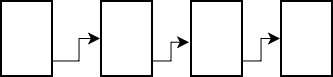
\includepdf[]{Chapter2/Figs/PDF/Diagramm1.pdf}
\begin{center}
\begin{figure}[h]
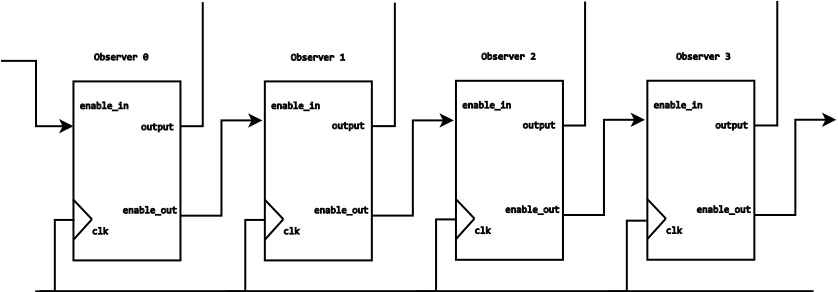
\includegraphics[width=450px]{Chapter2/Figs/Raster/Observer-stage.png}
\caption[Invariant Observer stages in cascade , m=4]{Example for m=4 Invariant Observer Stages concatenated in cascade. }
\label{fig:observerstages}
\end{figure}
\end{center}
This ensures,that these observers are starting delayed,in the meaning of time.\\
Signal \textbf{inc\_tau}(VDHL-Code~\ref{appendix:source:2},line 21) increments the input signal \textbf{invariance\_tau},which represents $\tau+1$ at every execution time.
The asynchronous part works immediately after every change of the system state.(VDHL-Code~\ref{appendix:source:2},line 25 and line 51)
In the following descriptions of the asynchronous parts,only temporary signals are changed,
but these signals transfer their values inside the synchronous part at every clock cycle,except \textbf{inc\_tau} and \textbf{enable\_logic}.
Every of these signals are indicated with "\_next" at the end of their names,but in the following descriptions only their register counterparts will be mentioned. 
\newline \newline
The process entity \textbf{comb\_cycle}(VDHL-Code~\ref{appendix:source:2},line 25) is the description of an internal clock counter which only counts up and down between values 0 and m.
The signal \textbf{cycle} is significant for checking the condition ``(clock mod m) = 0'' from Algorithm~\ref{alg:observerstage}.\\ \\
The process entity \textbf{comb\_logic} implements the real part of the algorithm.
Signal \textbf{count\_p} will be incremented in each clock cycle until it reaches $\tau+1$.
The counter should be initialised to zero (as indicated in the algorithm),but is incremented immediately at every clock cycle.(VDHL-Code~\ref{appendix:source:2},line 55)
Or in other words,if \textbf{count\_p} is reset to zero in a clock cycle,it will be incremented immediately in the "same" clock cycle. 
To demonstrate this fact we have an additional signal \textbf{count}, initialised with 1. 
But this signal is only for reasoning and will be reduced by a syntheses tool.  
The synchronous design is cumbersome in a way,which is due to the way of how the states change.
If the counter is supposed to be incremented after evaluating some conditions,this does not imply an immediate change of the counter.
To overcome this handicap the counter  \textbf{count\_p} is initialised to 2(VDHL-Code~\ref{appendix:source:2},line 56) which means,that 
at every clock cycle we check if the counter count\_p will reach a maximum at the next clock cycle. This enables us to change things on time. 
According to the Algorithm~\ref{alg:observerstage} at line 5,\textbf{count\_p} will only be reset if signal $W(\phi)$ has been evaluated as being not active in \textbf{comb\_cycle}. 
(VDHL-Code~\ref{appendix:source:2},line 56) \\\\
The first if-branch at line 53 of the VDHL-Code~\ref{appendix:source:2} checks two cases.
At first it will be checked if the clock passed m cycles or not and second if the signal \textbf{enable\_logic} is supposed to be active.
The first question is in term of Algorithm~\ref{alg:observerstage},line 2.
The second question concerns the signal \textbf{enable\_logic}. This signal combines \textbf{enable\_in} and \textbf{reset} in one signal. 
If signal \textbf{enable\_logic} is active,means that the observer stage is active and no reset condition happens.
The else-branch of the first if-branch at line 67  of the VDHL-Code~\ref{appendix:source:2} checks the condition in terms of  Algorithm~\ref{alg:observerstage},line 11.
The content of the if-branch (line 53) and the else-branch (67) are nearly the same,but there are two exceptions.
Inside the if-branch,beginning at line 54,the status of signal W($\phi$) will be checked,according to Algorithm~\ref{alg:observerstage},line 3.
And inside the else-branch at line 75,if m cycles are no yet passed and signal \textbf{count\_p} is already  at the maximum,
then signals \textbf{count\_p},\textbf{count} and \textbf{output} keep their old values.
The other parts of \textbf{comb\_cycle} are straightforward,if you compare it with the algorithm.In case the counter \textbf{count\_p} reaches the maximum,
the  \textbf{output} of the observer stage is activated. \\\\
Some points about the improvements made in that design,but it can also be seen as guidelines for further design cases.
It is very important that no Latches are built by the syntheses tool,so every if-branch must contain the same changes on the same signals.
A further point is to reduce the number of if-branches to a minimum. If-branches inside of an If branch extends signal paths and reduce the maximum clock design of the whole design.
In the next chapter we get an overview of the hardware realisation of the current design,which shows us a more visual view on that.

\chapter{My Third Chapter}

% **************************** Define Graphics Path **************************
\ifpdf
    \graphicspath{{Chapter3/Figs/Raster/}{Chapter3/Figs/PDF/}{Chapter3/Figs/}}
\else
    \graphicspath{{Chapter3/Figs/Vector/}{Chapter3/Figs/}}
\fi

\section{First Section of the Third Chapter}
And now I begin my third chapter here \dots

And now to cite some more people~\citet{Rea85,Ancey1996}

\subsection{First Subsection in the First Section}
\dots and some more 

\subsection{Second Subsection in the First Section}
\dots and some more \dots

\subsubsection{First subsub section in the second subsection}
\dots and some more in the first subsub section otherwise it all looks the same
doesn't it? well we can add some text to it \dots

\subsection{Third Subsection in the First Section}
\dots and some more \dots

\subsubsection{First subsub section in the third subsection}
\dots and some more in the first subsub section otherwise it all looks the same
doesn't it? well we can add some text to it and some more and some more and
some more and some more and some more and some more and some more \dots

\subsubsection{Second subsub section in the third subsection}
\dots and some more in the first subsub section otherwise it all looks the same
doesn't it? well we can add some text to it \dots

\section{Second Section of the Third Chapter}
and here I write more \dots

Now we can refer to the table using Table.~\ref{t:borders}.
\begin{table}[h]
\caption{Table with Borders}
\centering
\label{t:borders}
\begin{tabular}{|l|c| r|}

\hline
1 & 2 & 3 \\ \hline
4 & 5 & 6 \\ \hline
7 & 8 & 9 \\ \hline
\end{tabular}
\end{table}

\chapter{Experiments and Testing}

% **************************** Define Graphics Path **************************
\ifpdf
    \graphicspath{{Chapter3/Figs/Raster/}{Chapter3/Figs/PDF/}{Chapter3/Figs/}}
\else
    \graphicspath{{Chapter3/Figs/Vector/}{Chapter3/Figs/}}
\fi



%\chapter{Summary}
\label{chapter:5}
%% NO PERSONAL FORMS us,we,I
%% quotes use like : ``text''
%% after point,doublepoints and commas there must be a BLANK SPACE

% **************************** Define Graphics Path **************************
\ifpdf
    \graphicspath{{Chapter3/Figs/Raster/}{Chapter3/Figs/PDF/}{Chapter3/Figs/}}
\else
    \graphicspath{{Chapter3/Figs/Vector/}{Chapter3/Figs/}}
\fi

It was introduced a alternative version of an Invariant Observer from \cite{RTFMBJ13} which circumvents specifical design restrictions from \cite{RTFMBJ13}.
For example no restrictions on the evaluation time y for a proposition $\phi$. 
With the possiblity of a massively parallel constuction of the Observer Stages as part of a complete Invariant Observer which allows to evaluate a proposition $\phi$ 
at every clock cycle, it could result to a big performance step.
The Observer Stages are in way more flexible than in \cite{RTFMBJ13}, besides the possibility to change the Invariant $\tau$ during runtime. But these advantages should be
tested in a more detailed experiment and under real-time conditions.
Another point to mention is, that the experiments considered only the case that the Observer Stages are running in the same time domain like the system that evaluates the proposition $\phi$ to W($\phi$).
For example three clock cycles which passes for W($\phi$) are also the same three clock cycles for the Observer Stages. It came out, that a better resolution could be performed if
the frequency that drives the Observer Stages is multiple higher than the frequency of the system that evaluates W($\phi$).
For example if W($\phi$) is driven with 10Khz and the Observer Stages with 20Khz and a Invariance of $\tau = 2$ on W($\phi$) should be monitored, then the Observer Stages must observe a invariance
of $\tau = 4$ to meet the same time domain. That aspect should be considered in further real-time experiments. 
In \cite{RTFMBJ13} these two systems are acting together.
The Invariant Observer should be considered as a temporal operator which follows the specifications of ptMTL $\boxdot _{[ y,y+\tau ]}$ but with the restriction that it can not perform the observation of the 
invariance inside intervall [0,y], because the computation of proposition $\phi$ can not be immediately available.(remember y as the calculation time to calculate proposition $\phi$ to result W($\phi$ ))
Finally, the design approach of the Invariant Observer shows another possiblity to implement the other temporal operators from the Metric Temporal Logic like the ``Exists-Operator within Intervalls''.





%\include{Chapter6/chapter6}
%\include{Chapter7/chapter7}



% ********************************** Back Matter *******************************
% Backmatter should be commented out, if you are using appendices after References
%\backmatter 

% ********************************** Bibliography ******************************
\begin{spacing}{0.9}

% To use the conventional natbib style referencing
% Bibliography style previews: http://nodonn.tipido.net/bibstyle.php

%\bibliographystyle{apalike}
\bibliographystyle{plainnat} % use this to have URLs listed in References
\cleardoublepage
\bibliography{References/references} % Path to your References.bib file


% If you would like to use BibLaTeX for your references, pass `custombib' as 
% an option in the document class. The location of 'reference.bib' should be 
% specified in the preamble.tex file in the custombib section. 
% Comment out the lines related to natbib above and uncomment the following line.

% \printbibliography[heading=bibintoc, title={References}]


\end{spacing}

% ********************************** Appendices ********************************

\begin{appendices} % Using appendices environment for more functunality

% ******************************* Thesis Appendix A ********************************
\chapter{Source Implementation in VHDL} 
\label{appendix:1}
The following source Codes in this Appendix A shows the implementation of
the Invariant Observer. 
The Source Codes are written in VHDL 1993 and shows a description about the Behavioural Specification
of the design. \newline \newline
Observer.vhd is the entity specification of an Observer Stage and shows specifications about the input and outputs. 
Figure~\ref{fig:observerstages} shows us an excerpt of the input and output but at most how the several observer stages interact together.
\newline
Observer\_behave.vhd describes the exact behaviour of an observer stage. A detailed description of this behaviour is shown in  Chapter~\ref{chapter:sub:2}.
%\lstinputlisting[language=VHDL]{../../../../vhdl/Observer.vhd}

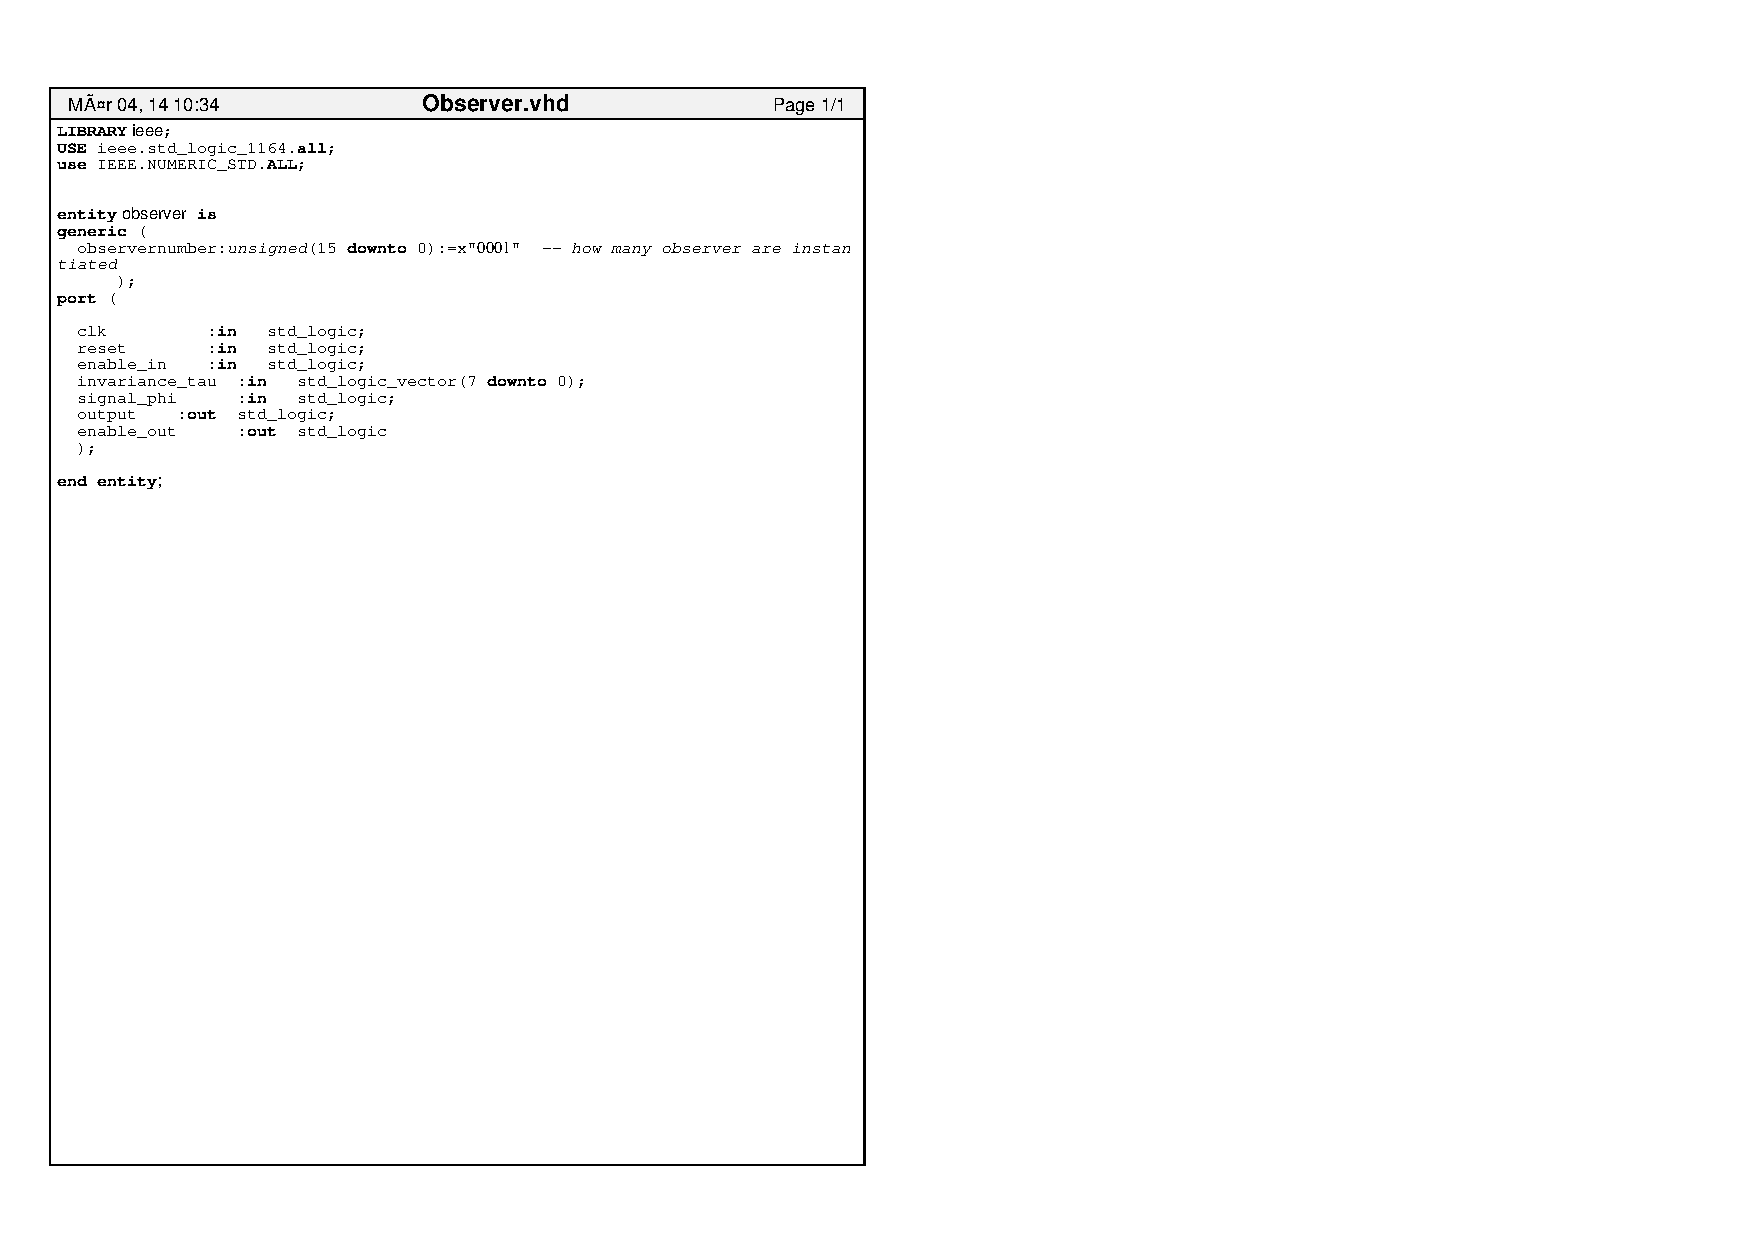
\includepdf[
 pages={-},
 nup=1x1,
 %landscape=false,
 %fitpaper=true,
 %noautoscale=false,
 turn=false,
 scale=1.6, 
 %trim= 0mm 0mm 0mm 0mm,
 clip=true,
 pagecommand={},
 %delta=0mm 0mm
 offset=-80mm 0mm
]{Appendix1/pdf/Observer.pdf}

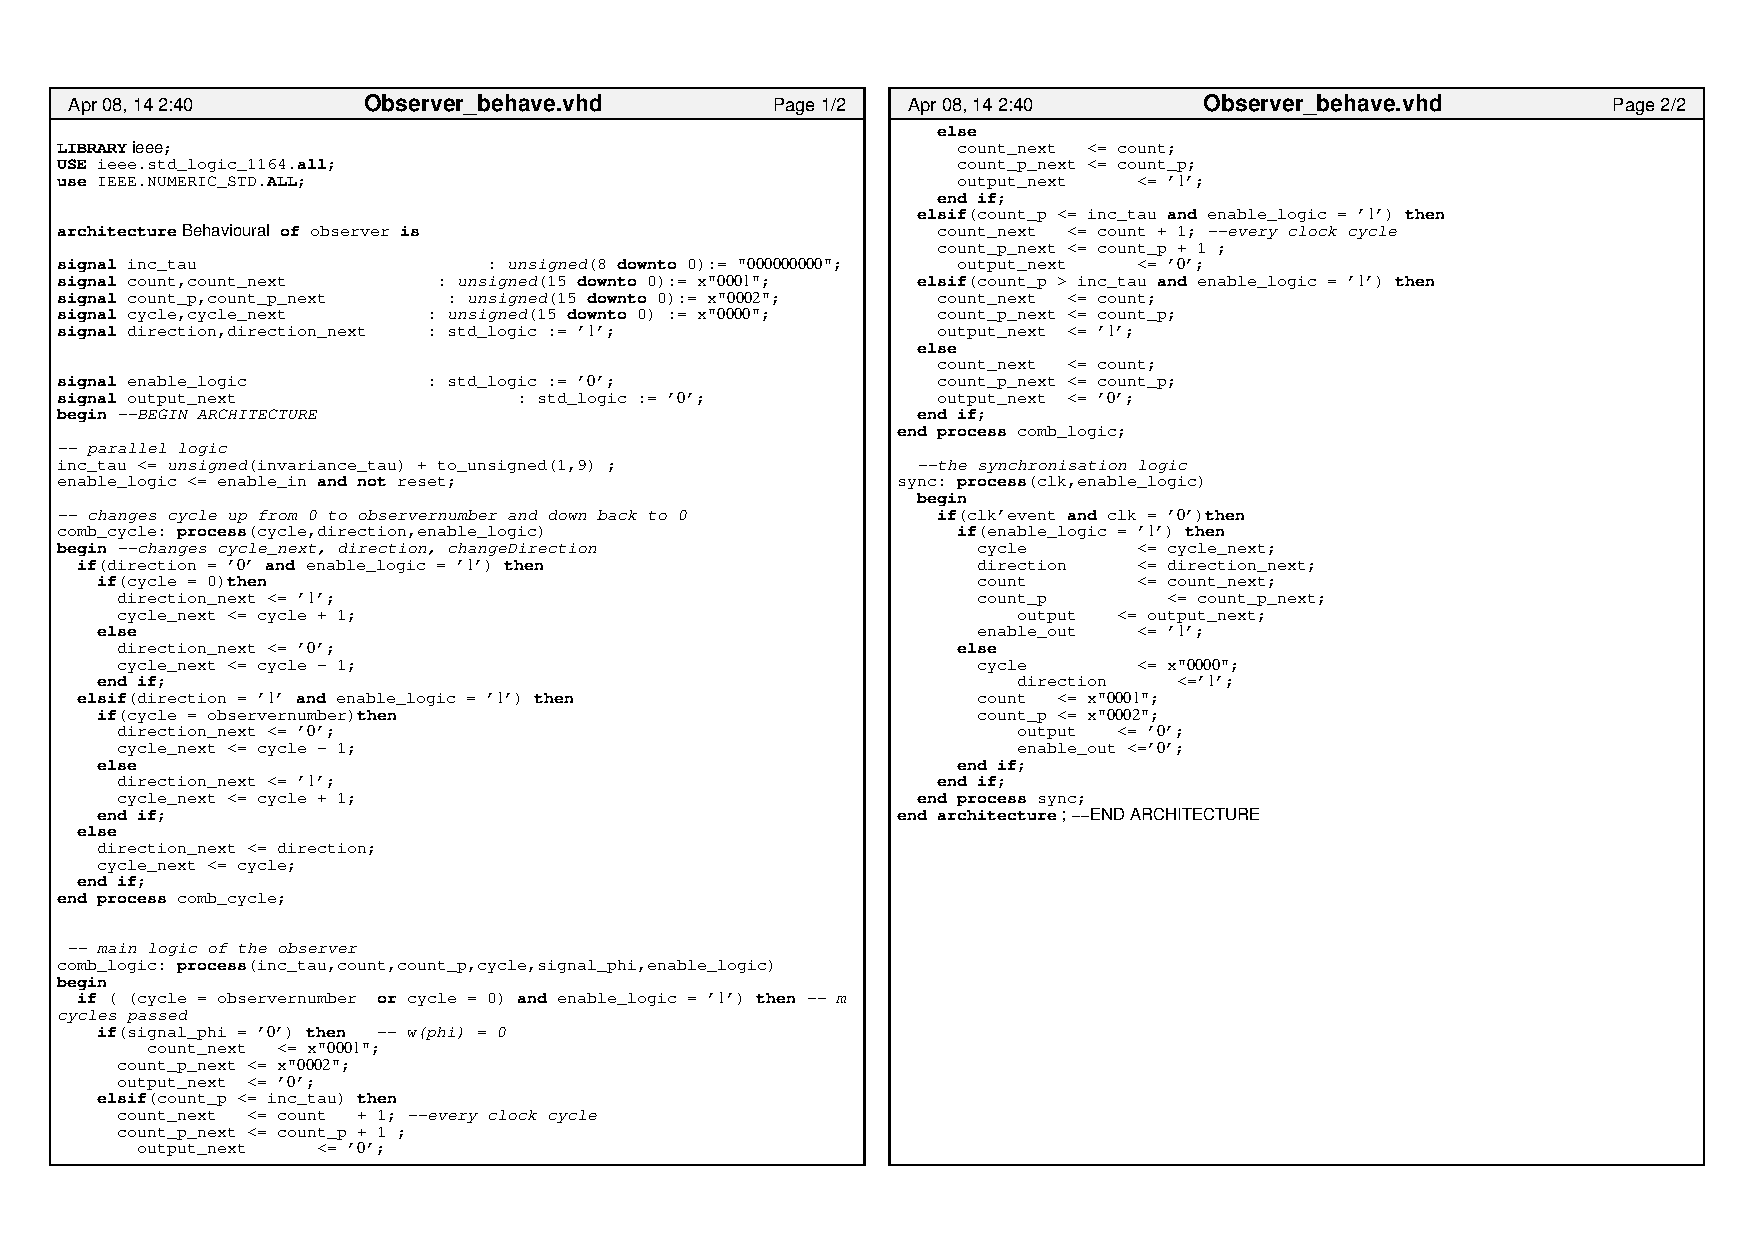
\includepdf[
 pages={-},
 nup=1x1,
 landscape=true,
 %fitpaper=true,
 noautoscale=false,
 turn=false,
 scale=0.9,
 %trim= 0mm 0mm 0mm 0mm,
 clip=true,
 pagecommand={},
 %delta=0mm 0mm
 %offset=-80mm 0mm
]{Appendix1/pdf/Observer_behave.pdf}

% ******************************* Thesis Appendix B ********************************

\chapter{Register Transfer Level Design View}
\label{appendix:2}

\begin{figure}[h]
\centering
%\hspace{3.0cm}
%\vspace{-5cm}
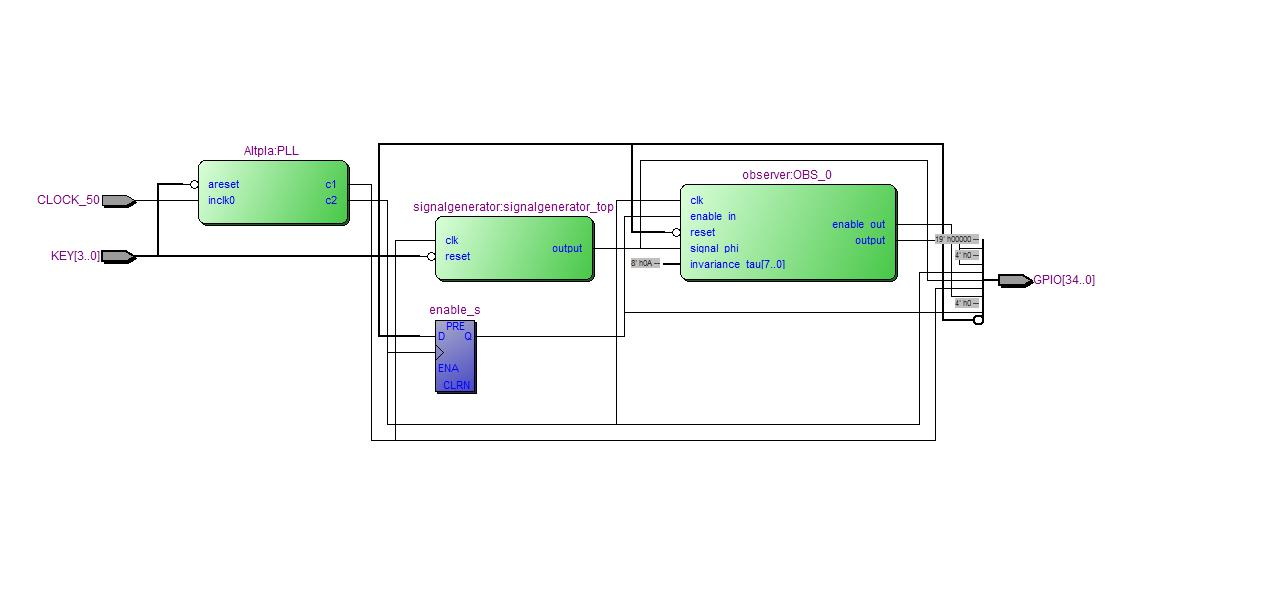
\includegraphics[width=650px,height=300px,angle=-90]{../../pictures/20.02.2014/TOP.jpg}
%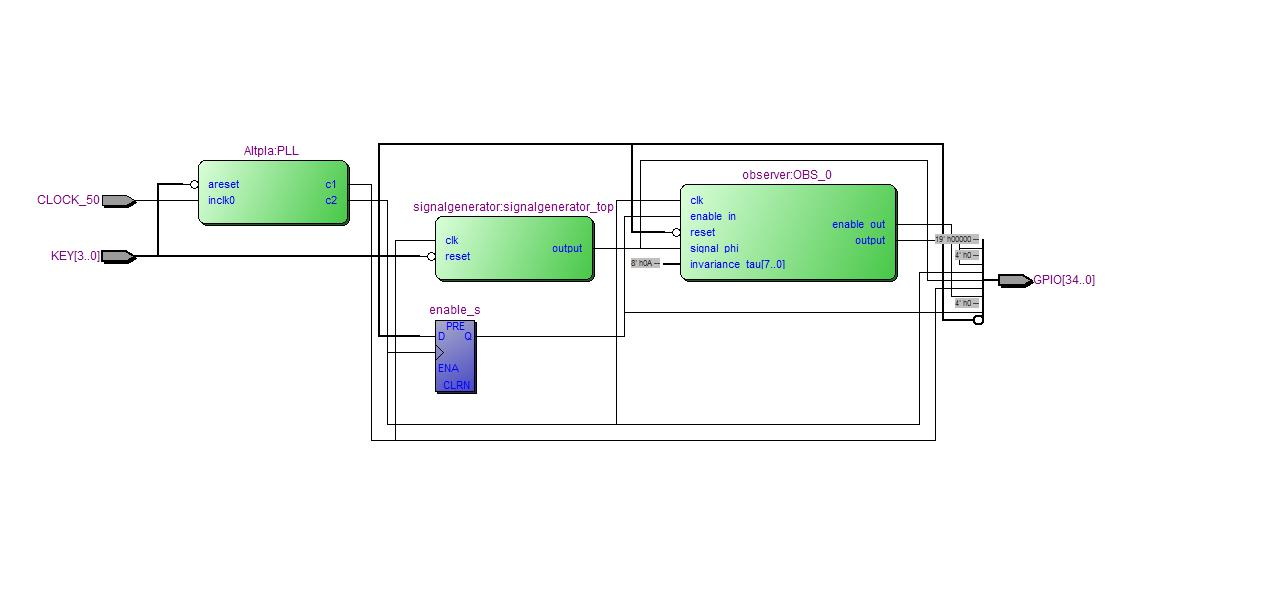
\includegraphics[height]{../../pictures/20.02.2014/TOP.jpg}
\caption[TOP Design of the First Version]{Illustration of the TOP Design of the first correct version,but without improvements}
\label{fig:version:one:top}
\end{figure}

\begin{figure}[h]
\centering
%\hspace{3.0cm}
%\vspace{-5cm}
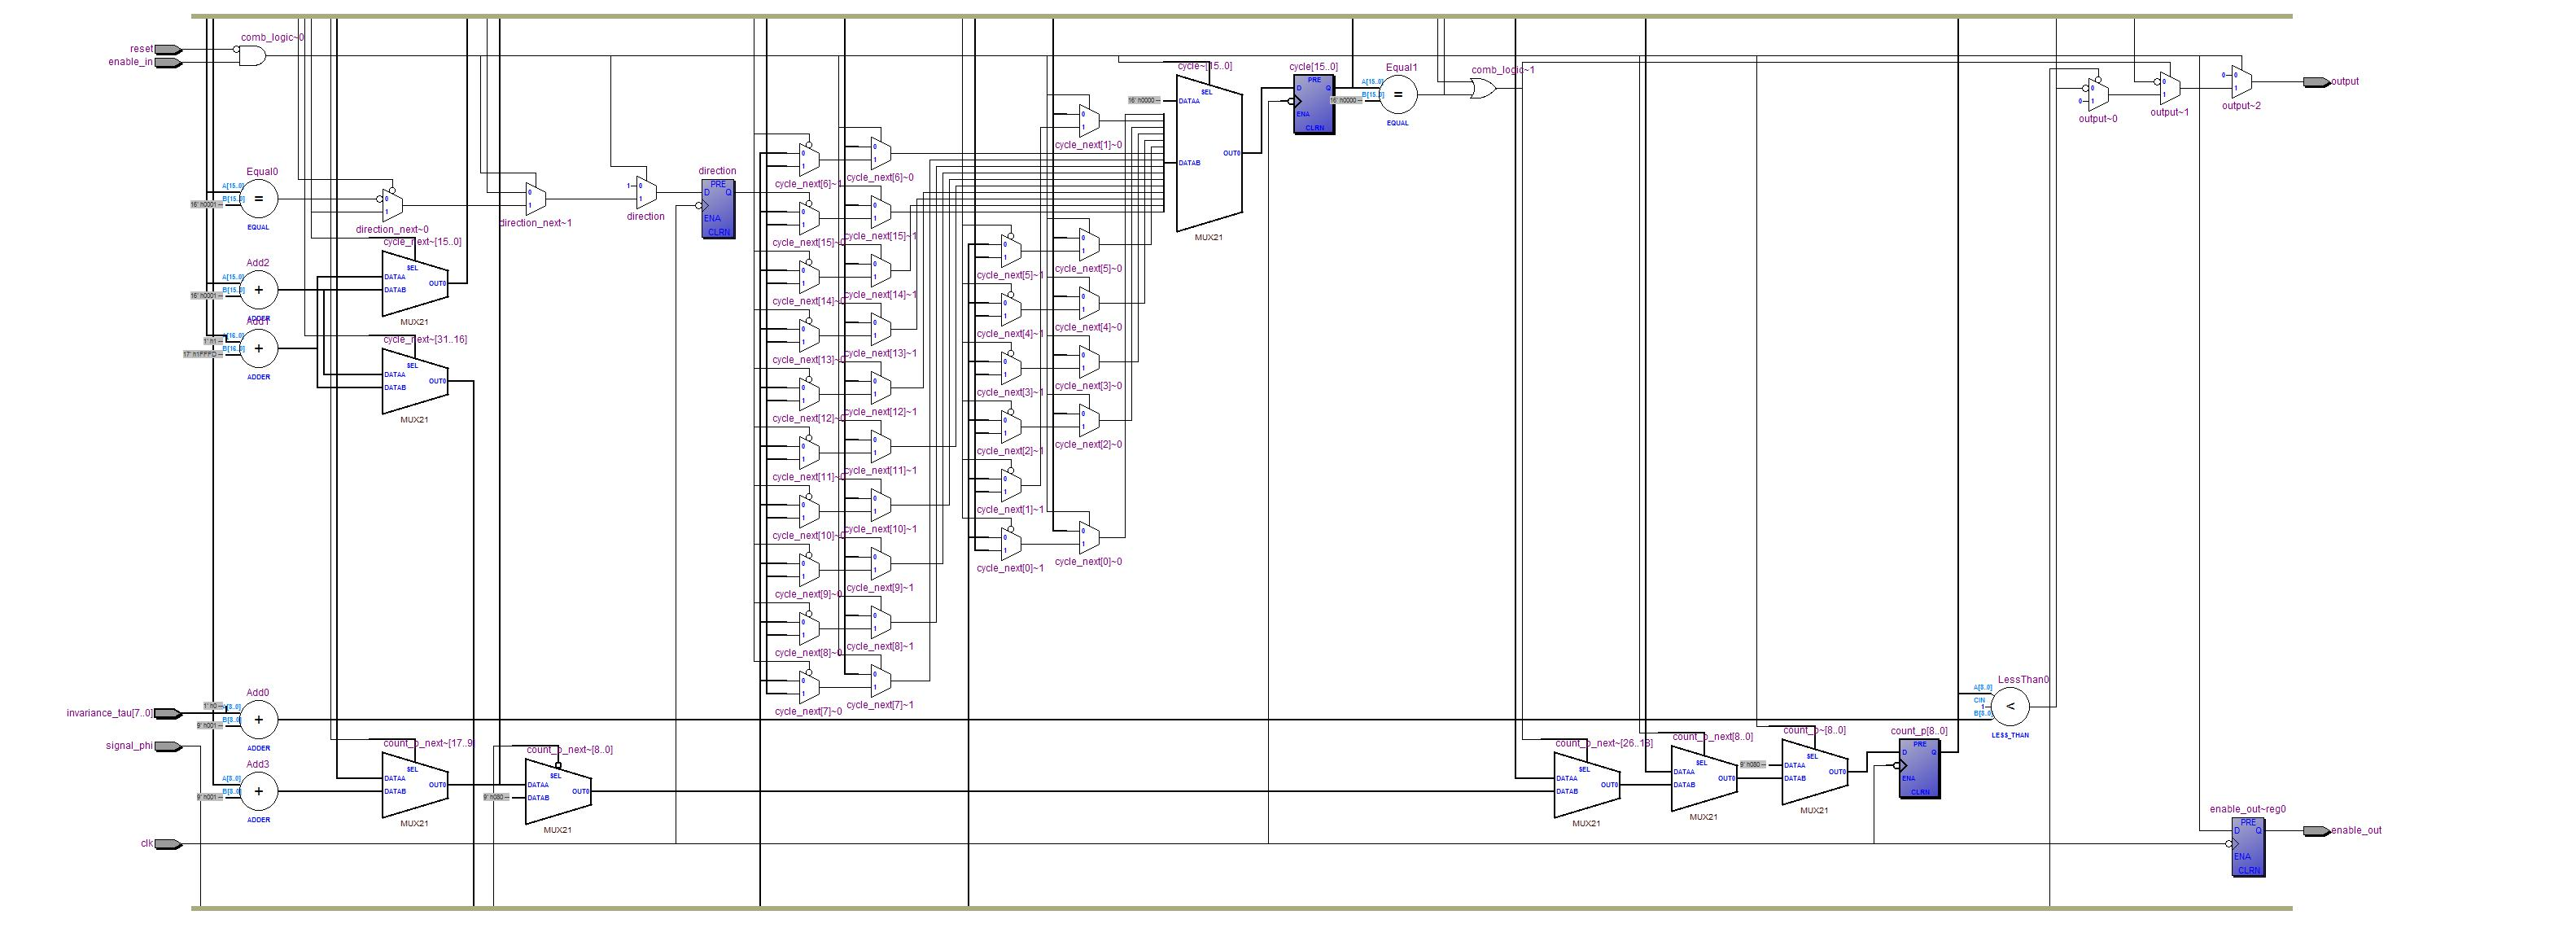
\includegraphics[width=650px,height=300px,angle=-90]{../../pictures/20.02.2014/observer_OBS_0.jpg}
%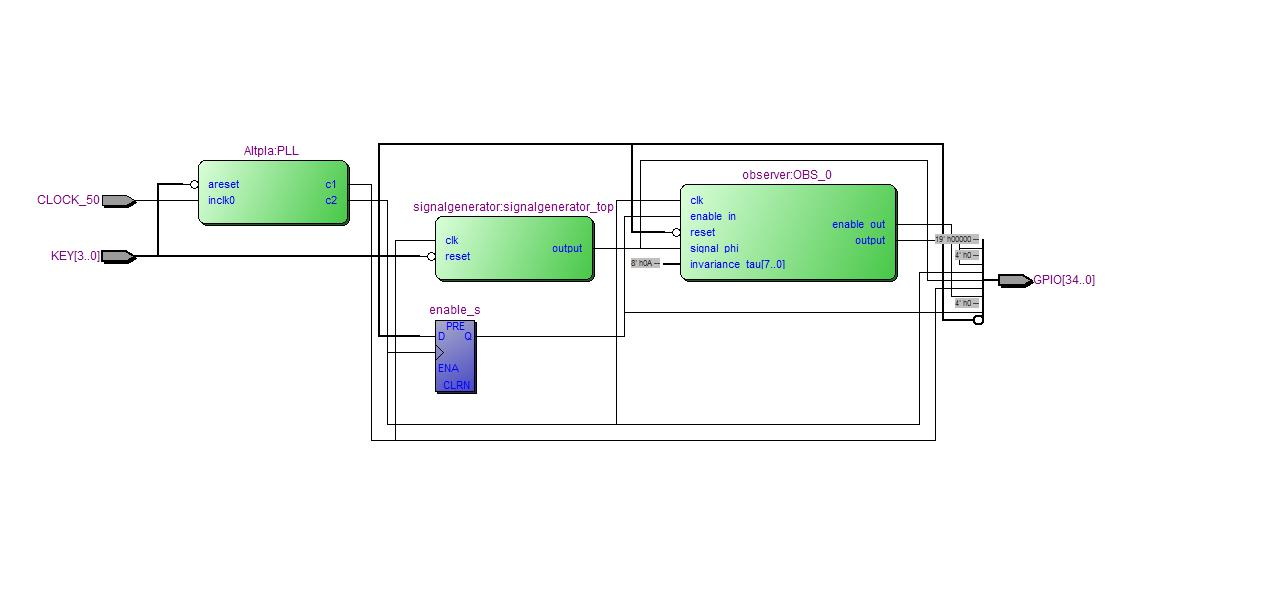
\includegraphics[height]{../../pictures/20.02.2014/TOP.jpg}
\caption[Observer Design of the First Version]{Illustration of the Observer Design of the first correct version,but without improvements}
\label{fig:version:one:obs}
\end{figure}

\begin{figure}[h]
\centering
%\hspace{3.0cm}
%\vspace{-5cm}
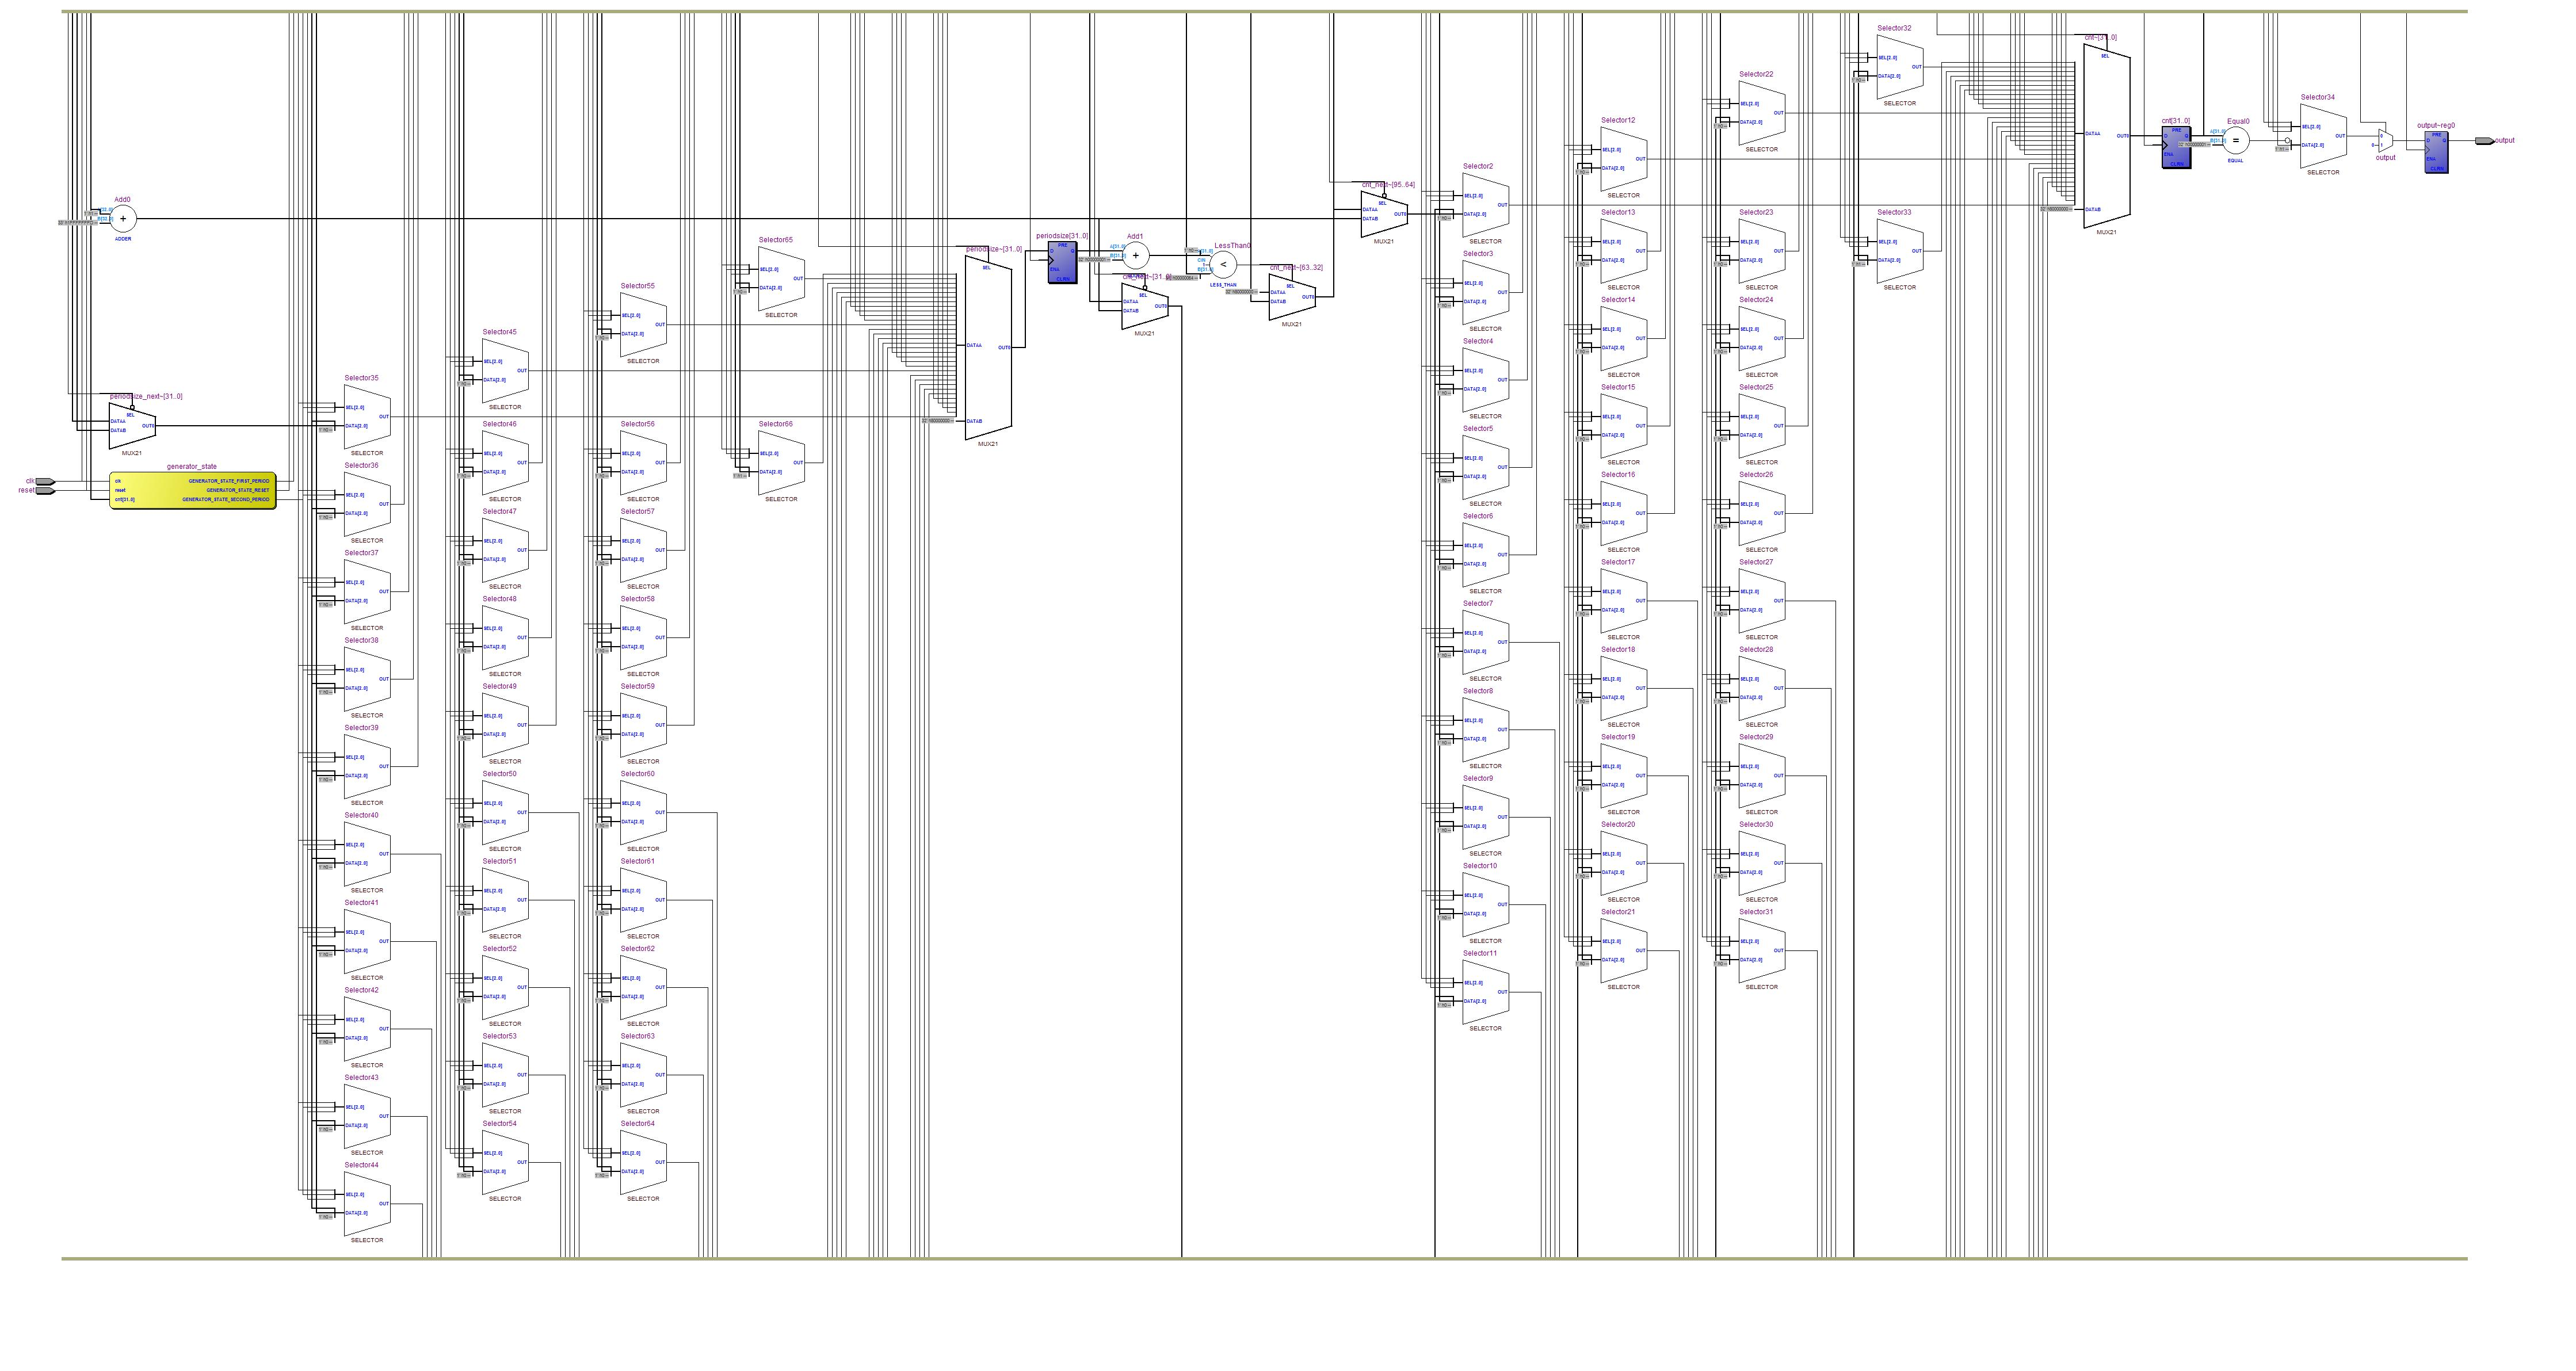
\includegraphics[width=650px,height=300px,angle=-90]{../../pictures/20.02.2014/signalgenerator_signalgenerator_top.jpg}
%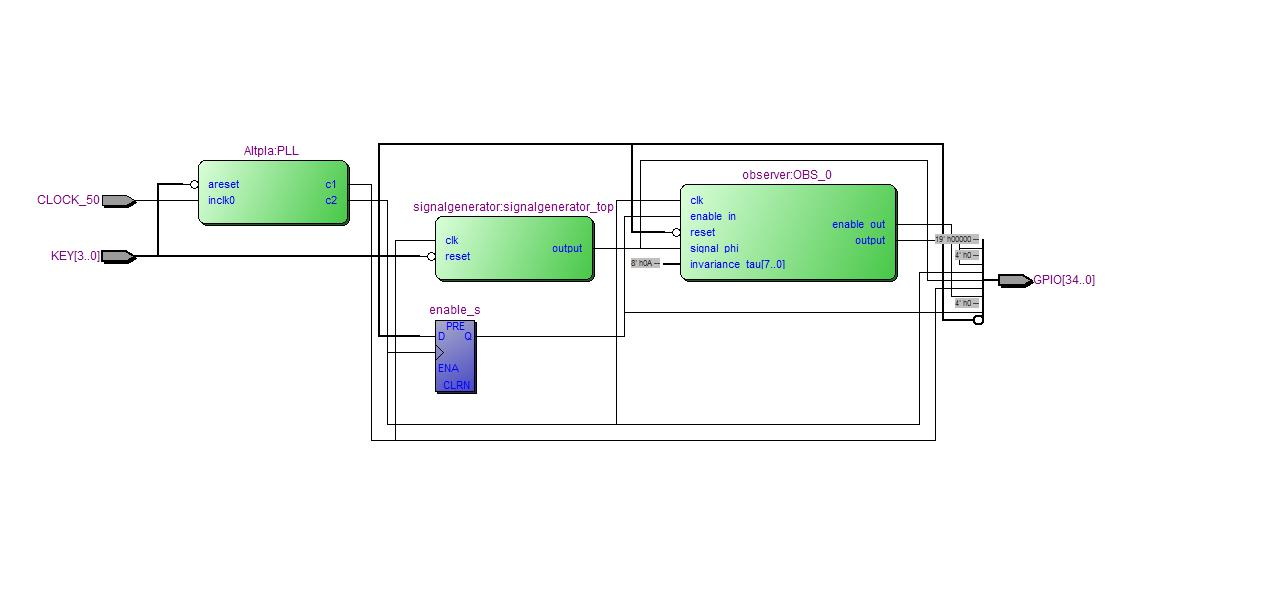
\includegraphics[height]{../../pictures/20.02.2014/TOP.jpg}
\caption[Signalgenerator of the First Version]{Illustration of the Signalgenerator of the first correct version,but without improvements}
\label{fig:version:one:sig}
\end{figure}

% ******************************* Thesis Appendix C ********************************

\chapter{Register Transfer Level Design View}
\label{appendix:3}
\section{Design of the First Version}
\label{appendix:3:section:1}
\begin{figure}[]
\centering
%\hspace{3.0cm}
%\vspace{-5cm}
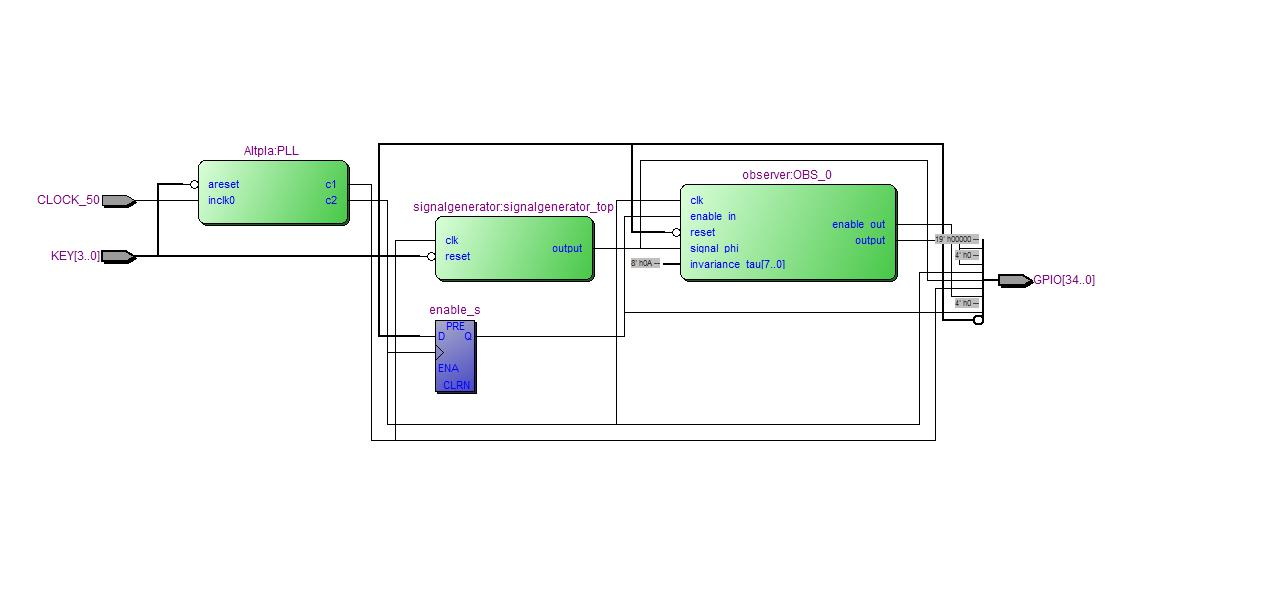
\includegraphics[width=650px,height=300px,angle=-90]{../../pictures/20.02.2014/TOP.jpg}
%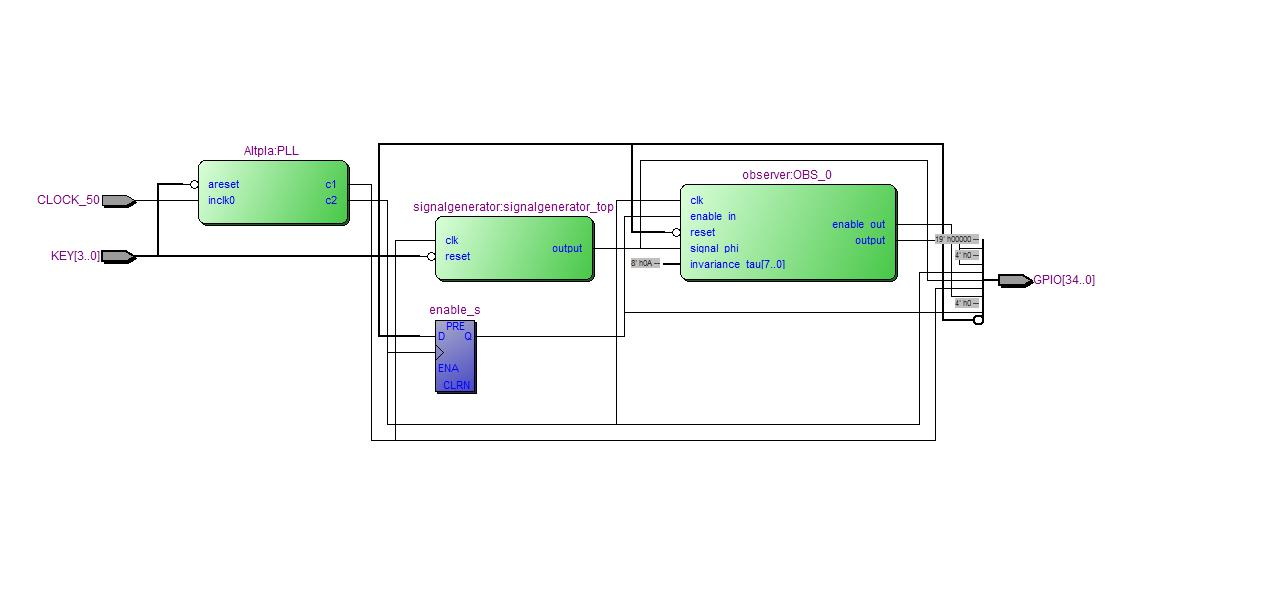
\includegraphics[height]{../../pictures/20.02.2014/TOP.jpg}
\caption[TOP Design of the First Version]{Illustration of the TOP Design of the first correct version,but without improvements}
\label{fig:version:one:top}
\end{figure}

\begin{figure}[]
\centering
%\hspace{3.0cm}
%\vspace{-5cm}
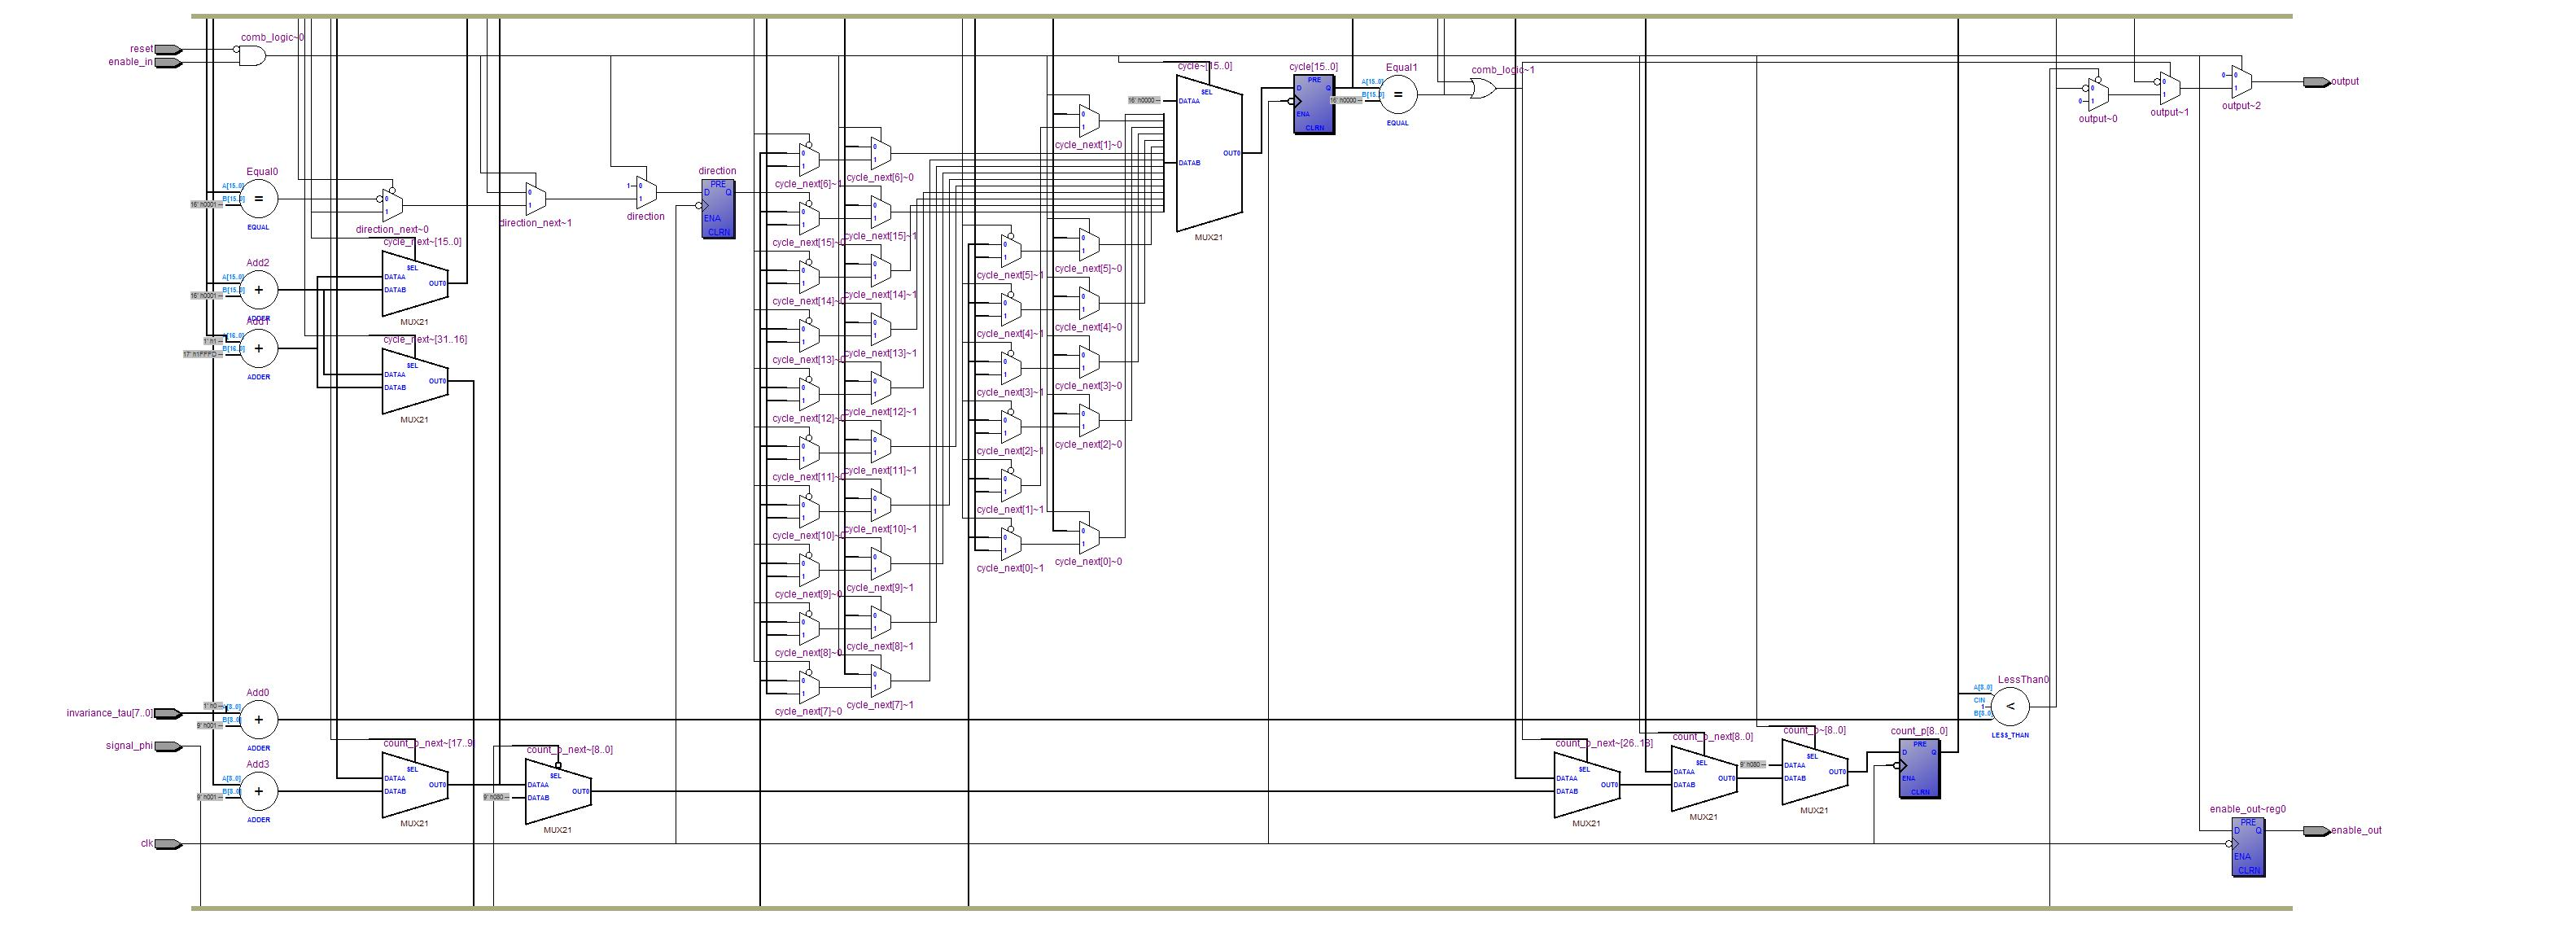
\includegraphics[width=650px,height=300px,angle=-90]{../../pictures/20.02.2014/observer_OBS_0.jpg}
%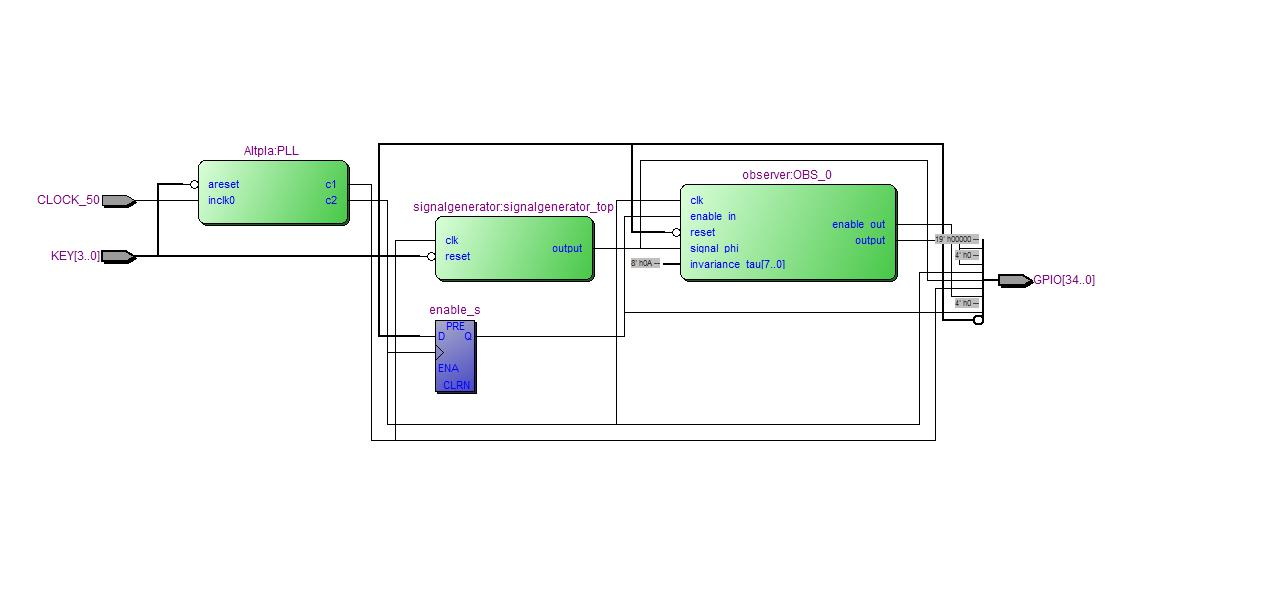
\includegraphics[height]{../../pictures/20.02.2014/TOP.jpg}
\caption[Observer Design of the First Version]{Illustration of the Observer Design of the first correct version,but without improvements}
\label{fig:version:one:obs}
\end{figure}

\begin{figure}[]
\centering
%\hspace{3.0cm}
%\vspace{-5cm}
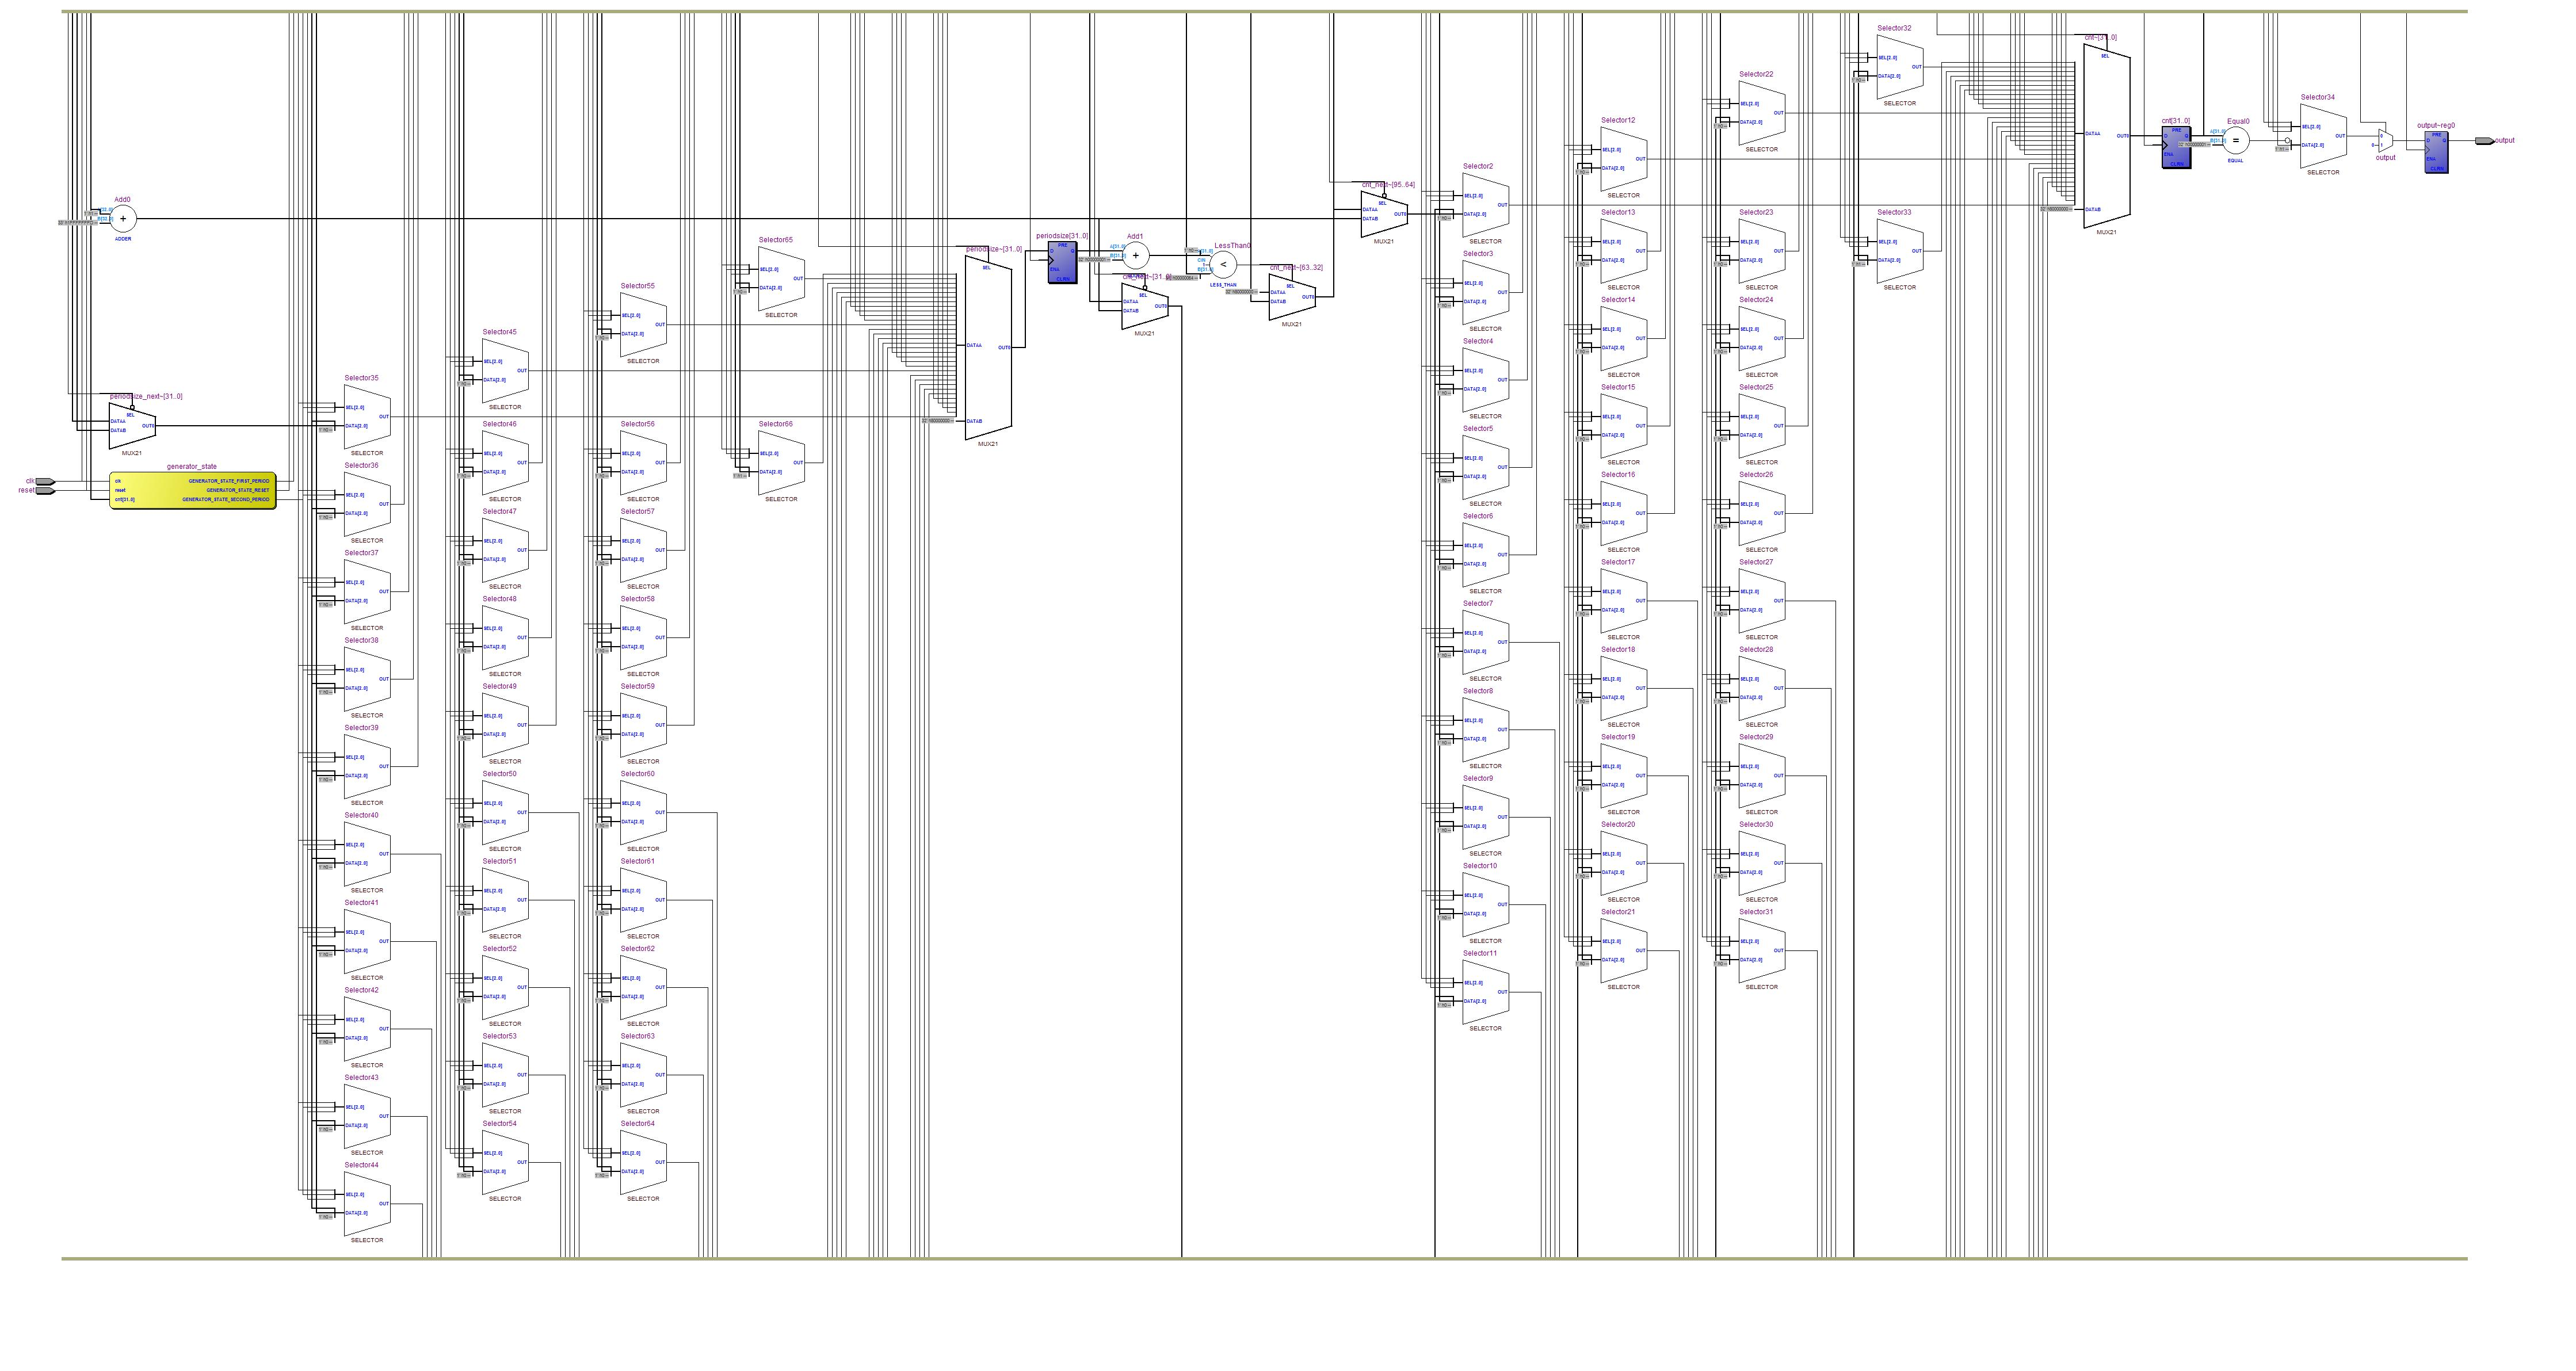
\includegraphics[width=650px,height=300px,angle=-90]{../../pictures/20.02.2014/signalgenerator_signalgenerator_top.jpg}
%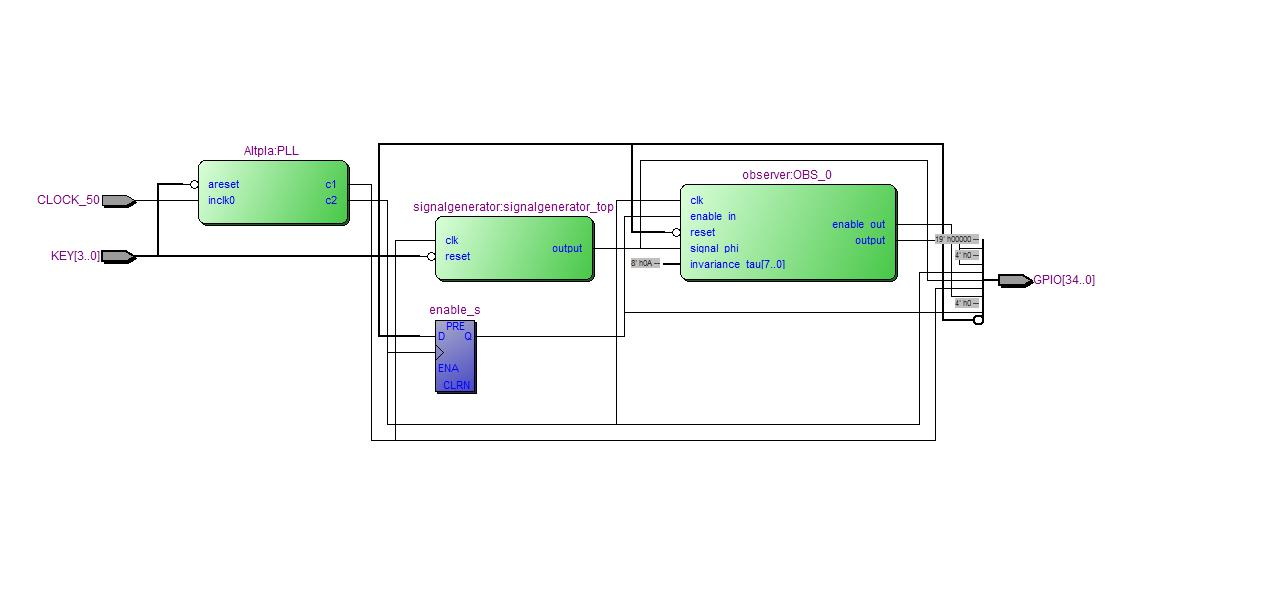
\includegraphics[height]{../../pictures/20.02.2014/TOP.jpg}
\caption[Signalgenerator of the First Version]{Illustration of the Signalgenerator of the first correct version,but without improvements}
\label{fig:version:one:sig}
\end{figure}

\section{Design of the most performant Version}
\label{appendix:3:section:2}


\begin{figure}[]
\centering
%\hspace{3.0cm}
%\vspace{-5cm}
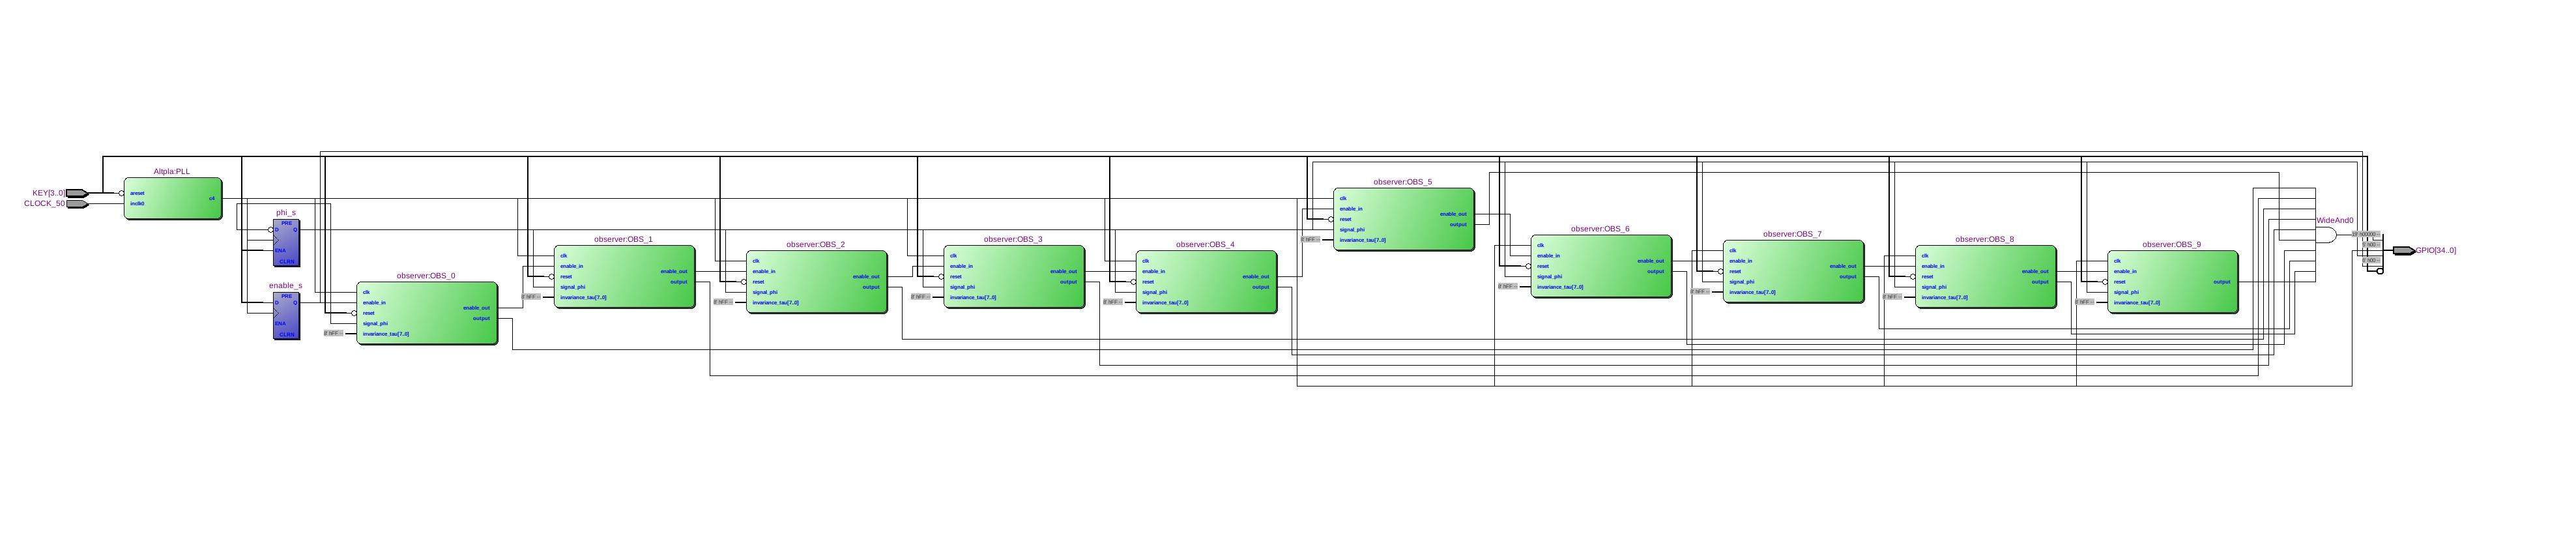
\includegraphics[width=650px,height=300px,angle=-90]{../../pictures/13.06.2014/plain_generator/200Mhz/10OBS/TOP_only_10Observer.jpg}
%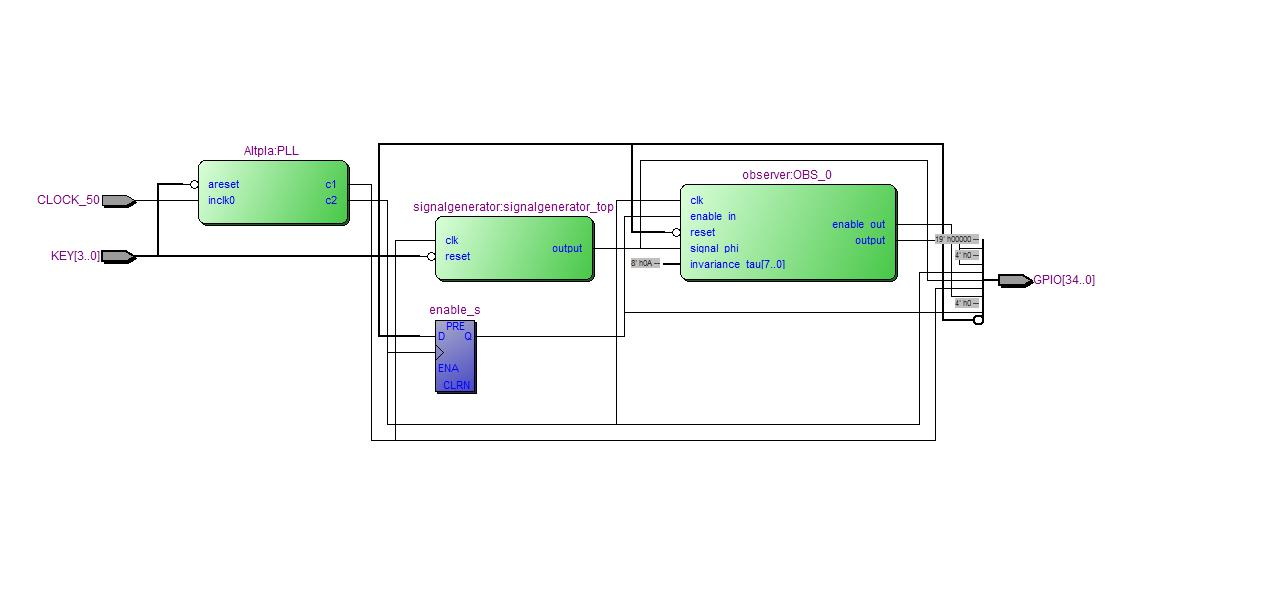
\includegraphics[height]{../../pictures/20.02.2014/TOP.jpg}
\caption[TOP Design of the Final Version]{Illustration of the TOP Design with the the best performance}
\label{fig:version:final:top}
\end{figure}

\begin{figure}[]
\centering
%\hspace{3.0cm}
%\vspace{-5cm}
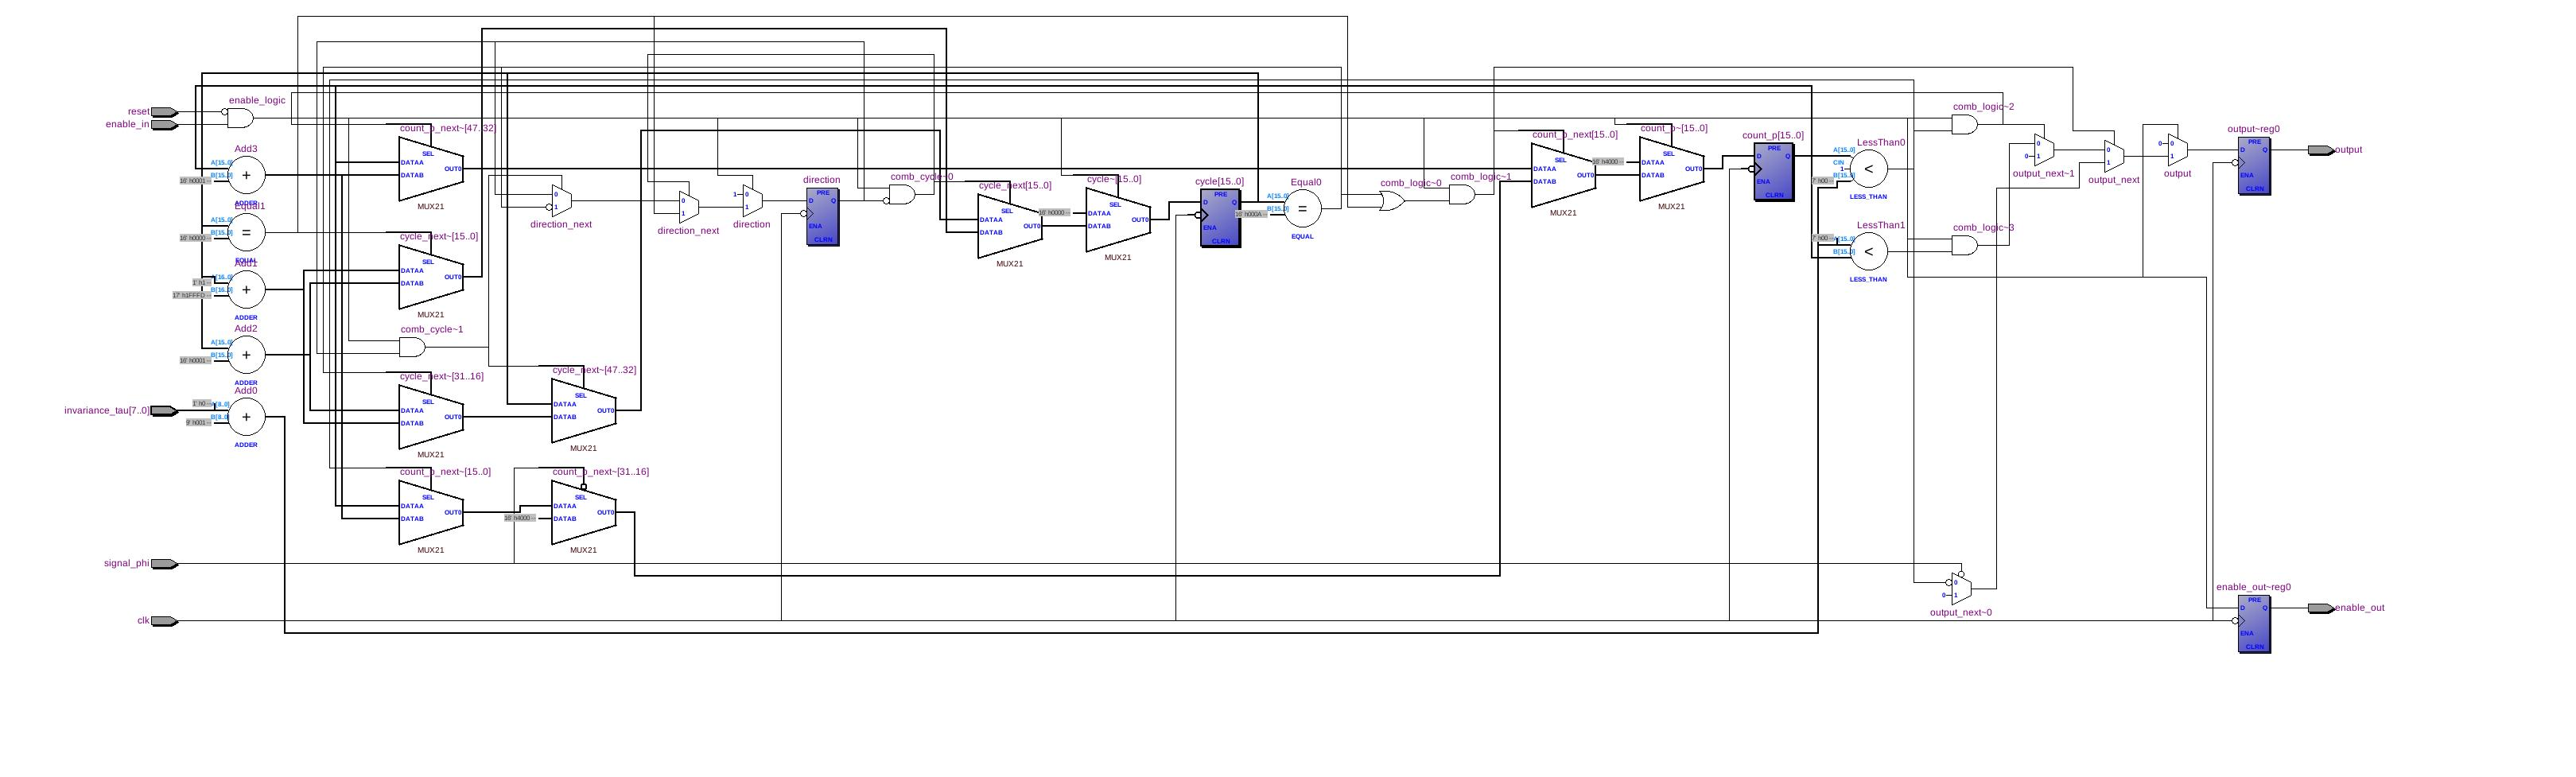
\includegraphics[width=650px,height=300px,angle=-90]{../../pictures/13.06.2014/plain_generator/200Mhz/10OBS/observer_OBS_0.jpg}
%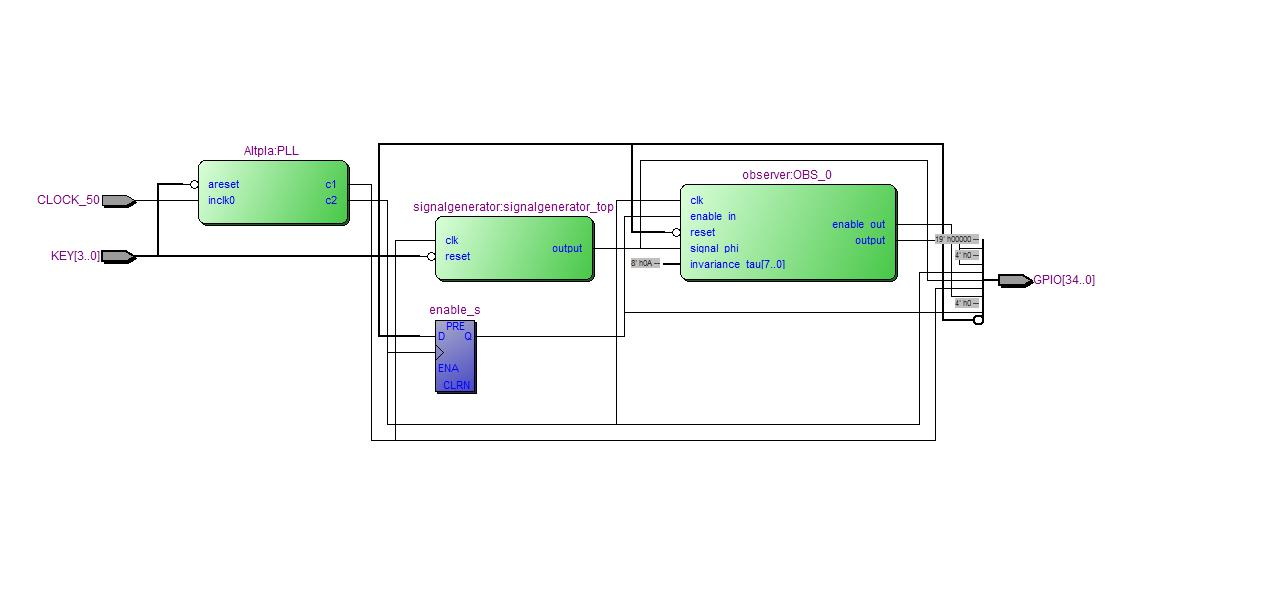
\includegraphics[height]{../../pictures/20.02.2014/TOP.jpg}
\caption[Observer 0 of the Final Version]{Illustration of the Observer 0 from 9 }
\label{fig:version:final:obs:0}
\end{figure}


\begin{figure}[]
\centering
%\hspace{3.0cm}
%\vspace{-5cm}
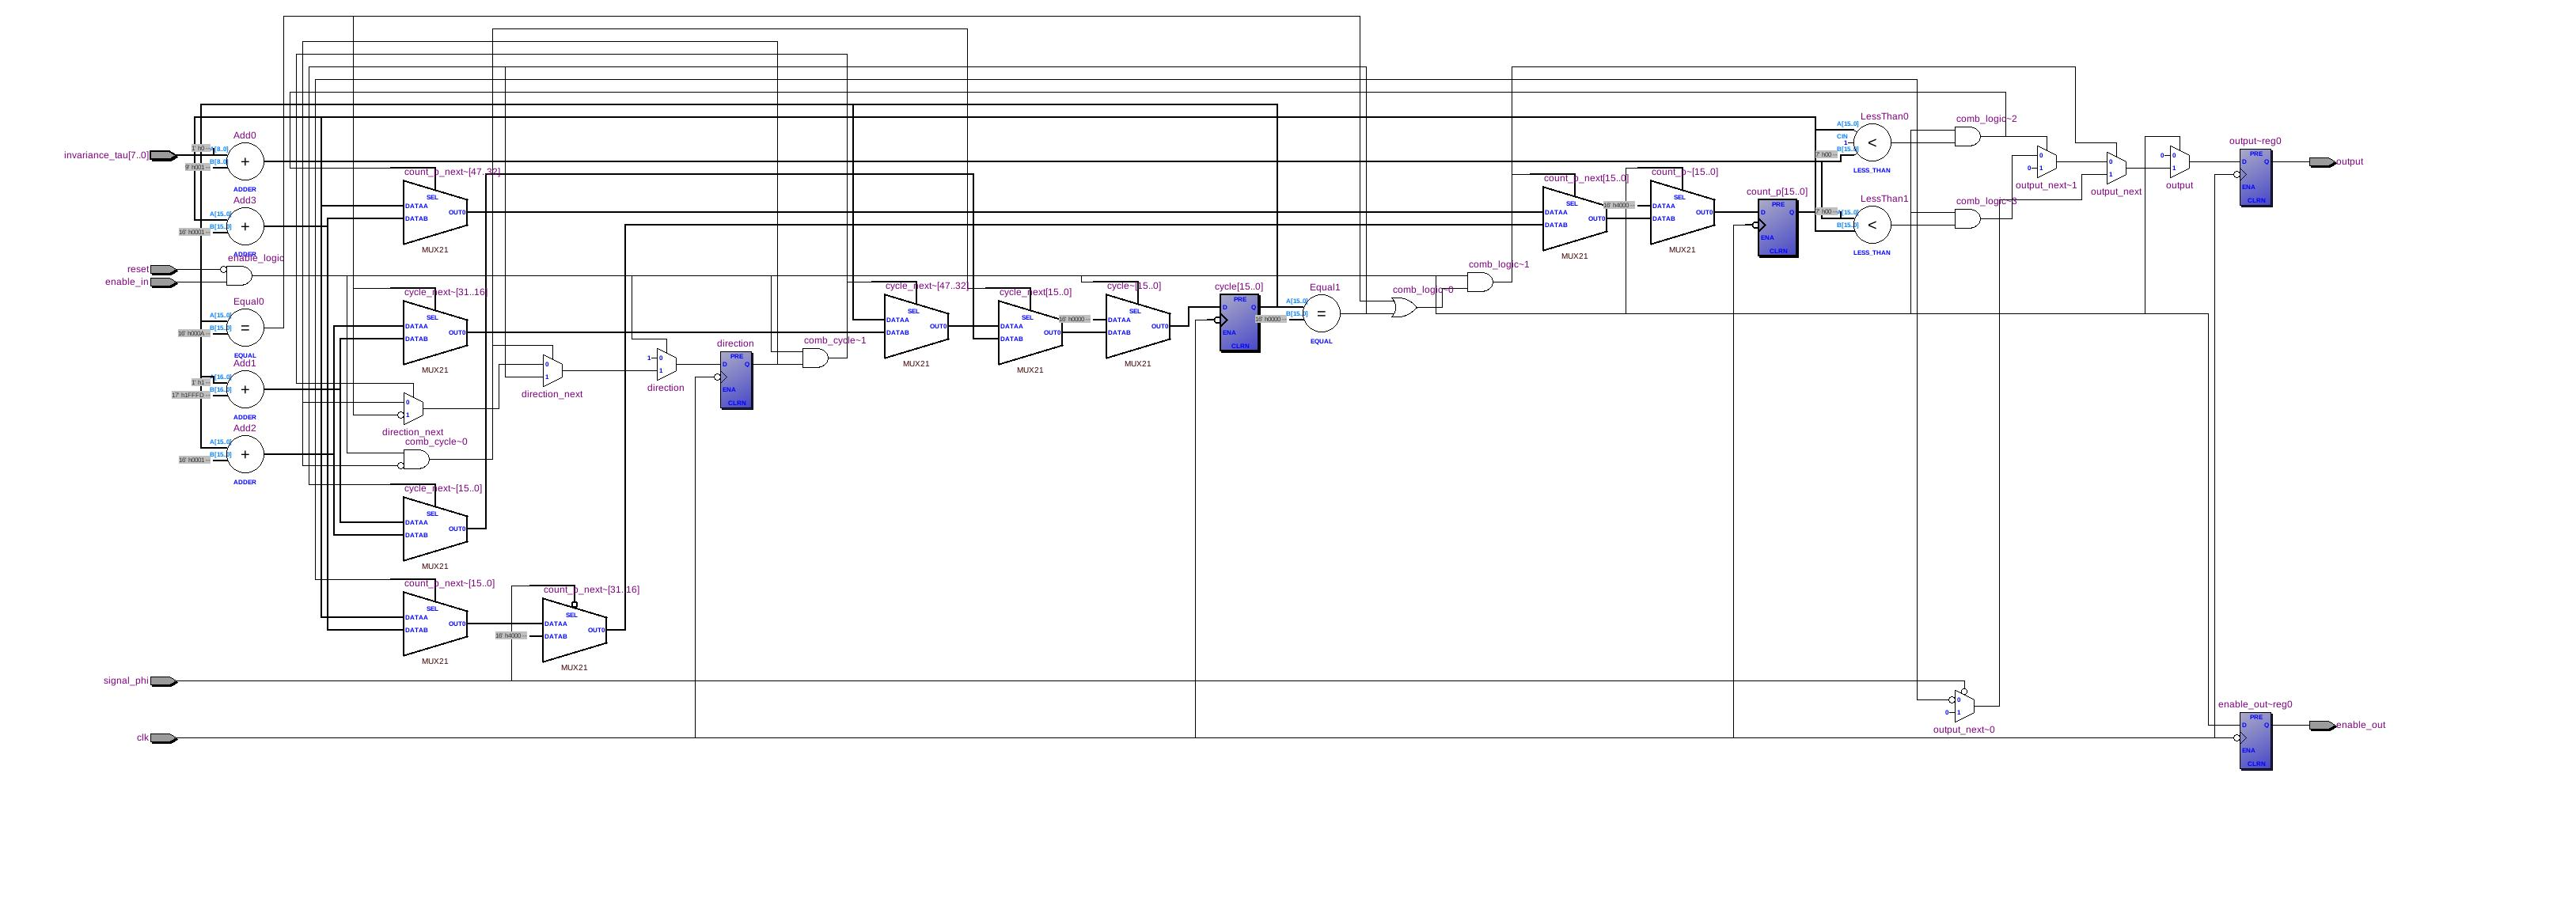
\includegraphics[width=650px,height=300px,angle=-90]{../../pictures/13.06.2014/plain_generator/200Mhz/10OBS/observer_OBS_5.jpg}
%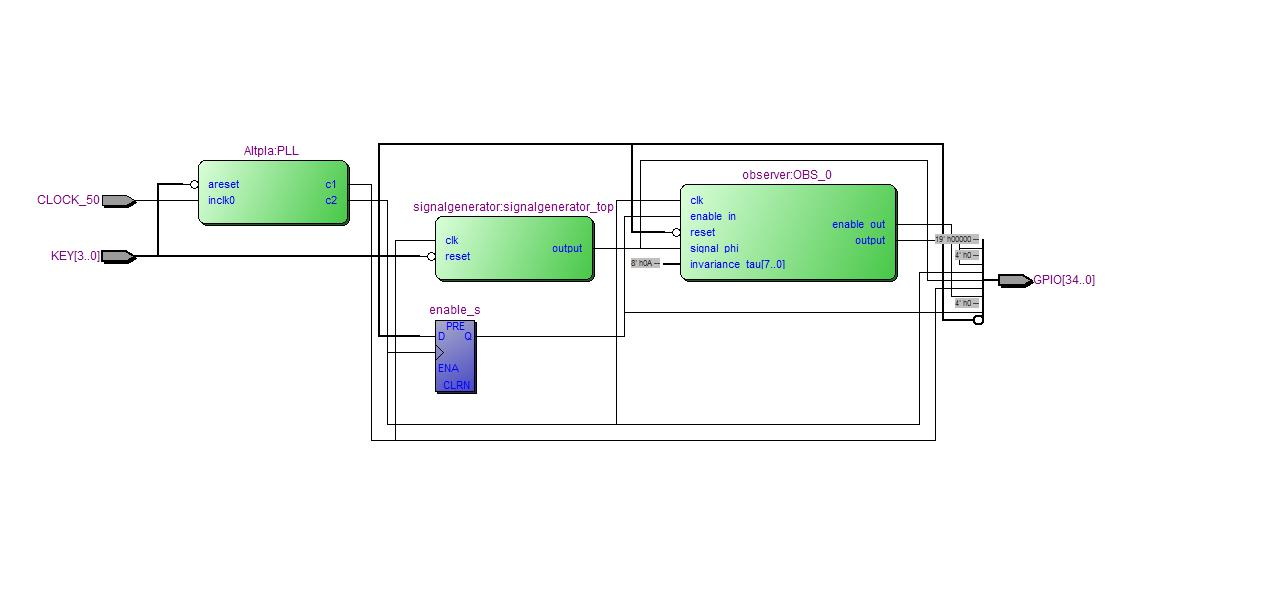
\includegraphics[height]{../../pictures/20.02.2014/TOP.jpg}
\caption[Observer 5  of the Final Version]{Illustration of the Observer 0 from 9 }
\label{fig:version:final:obs:5}
\end{figure}


\begin{figure}[]
\centering
%\hspace{3.0cm}
%\vspace{-5cm}
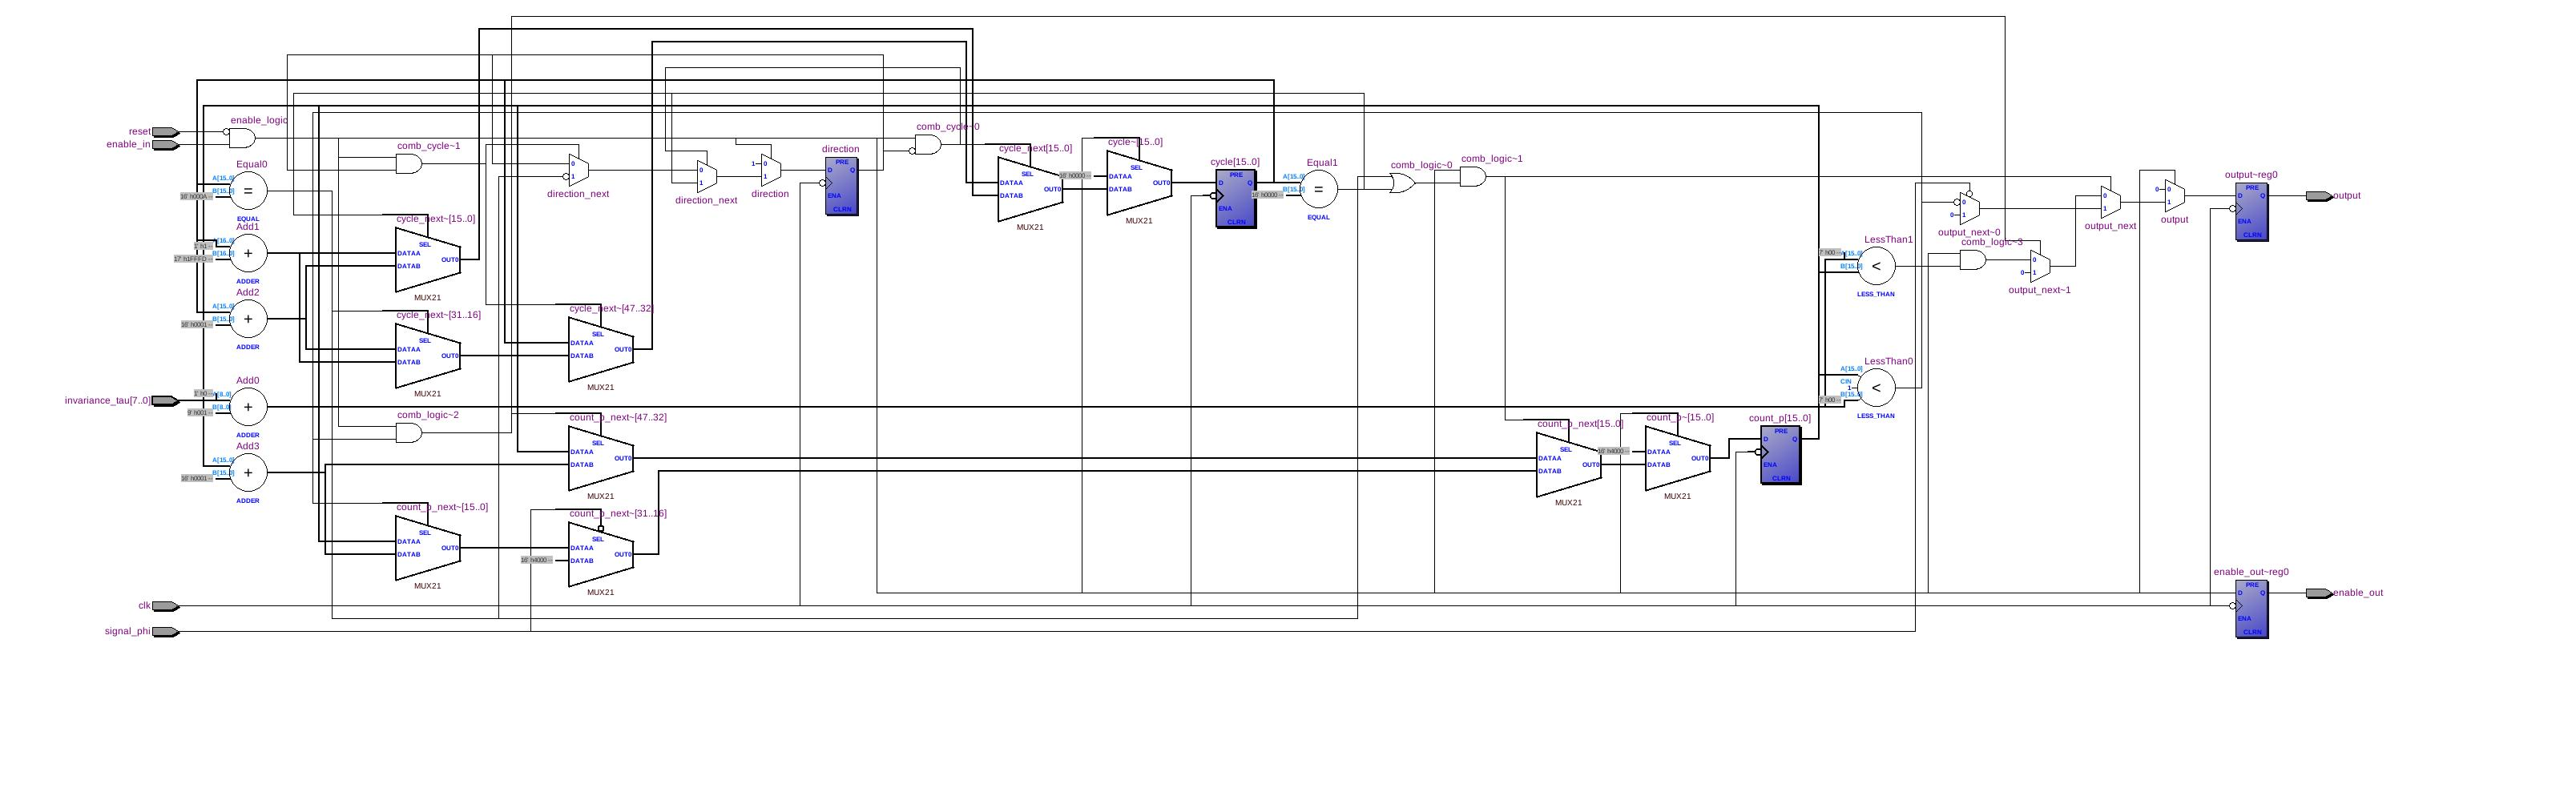
\includegraphics[width=650px,height=300px,angle=-90]{../../pictures/13.06.2014/plain_generator/200Mhz/10OBS/observer_OBS_9.jpg}
%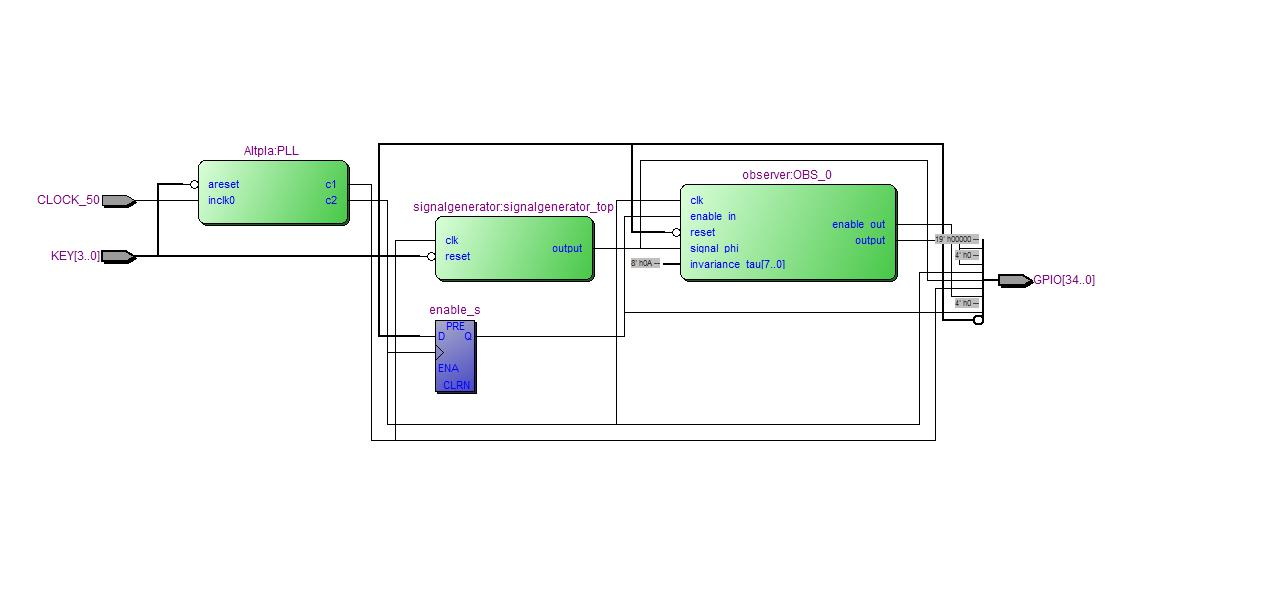
\includegraphics[height]{../../pictures/20.02.2014/TOP.jpg}
\caption[Observer 9  of the Final Version]{Illustration of the Observer 5 from 9 }
\label{fig:version:final:obs:9}
\end{figure}


% ******************************* Thesis Appendix D ********************************

\chapter{Datasheets and Descriptions}
\label{appendix:4}
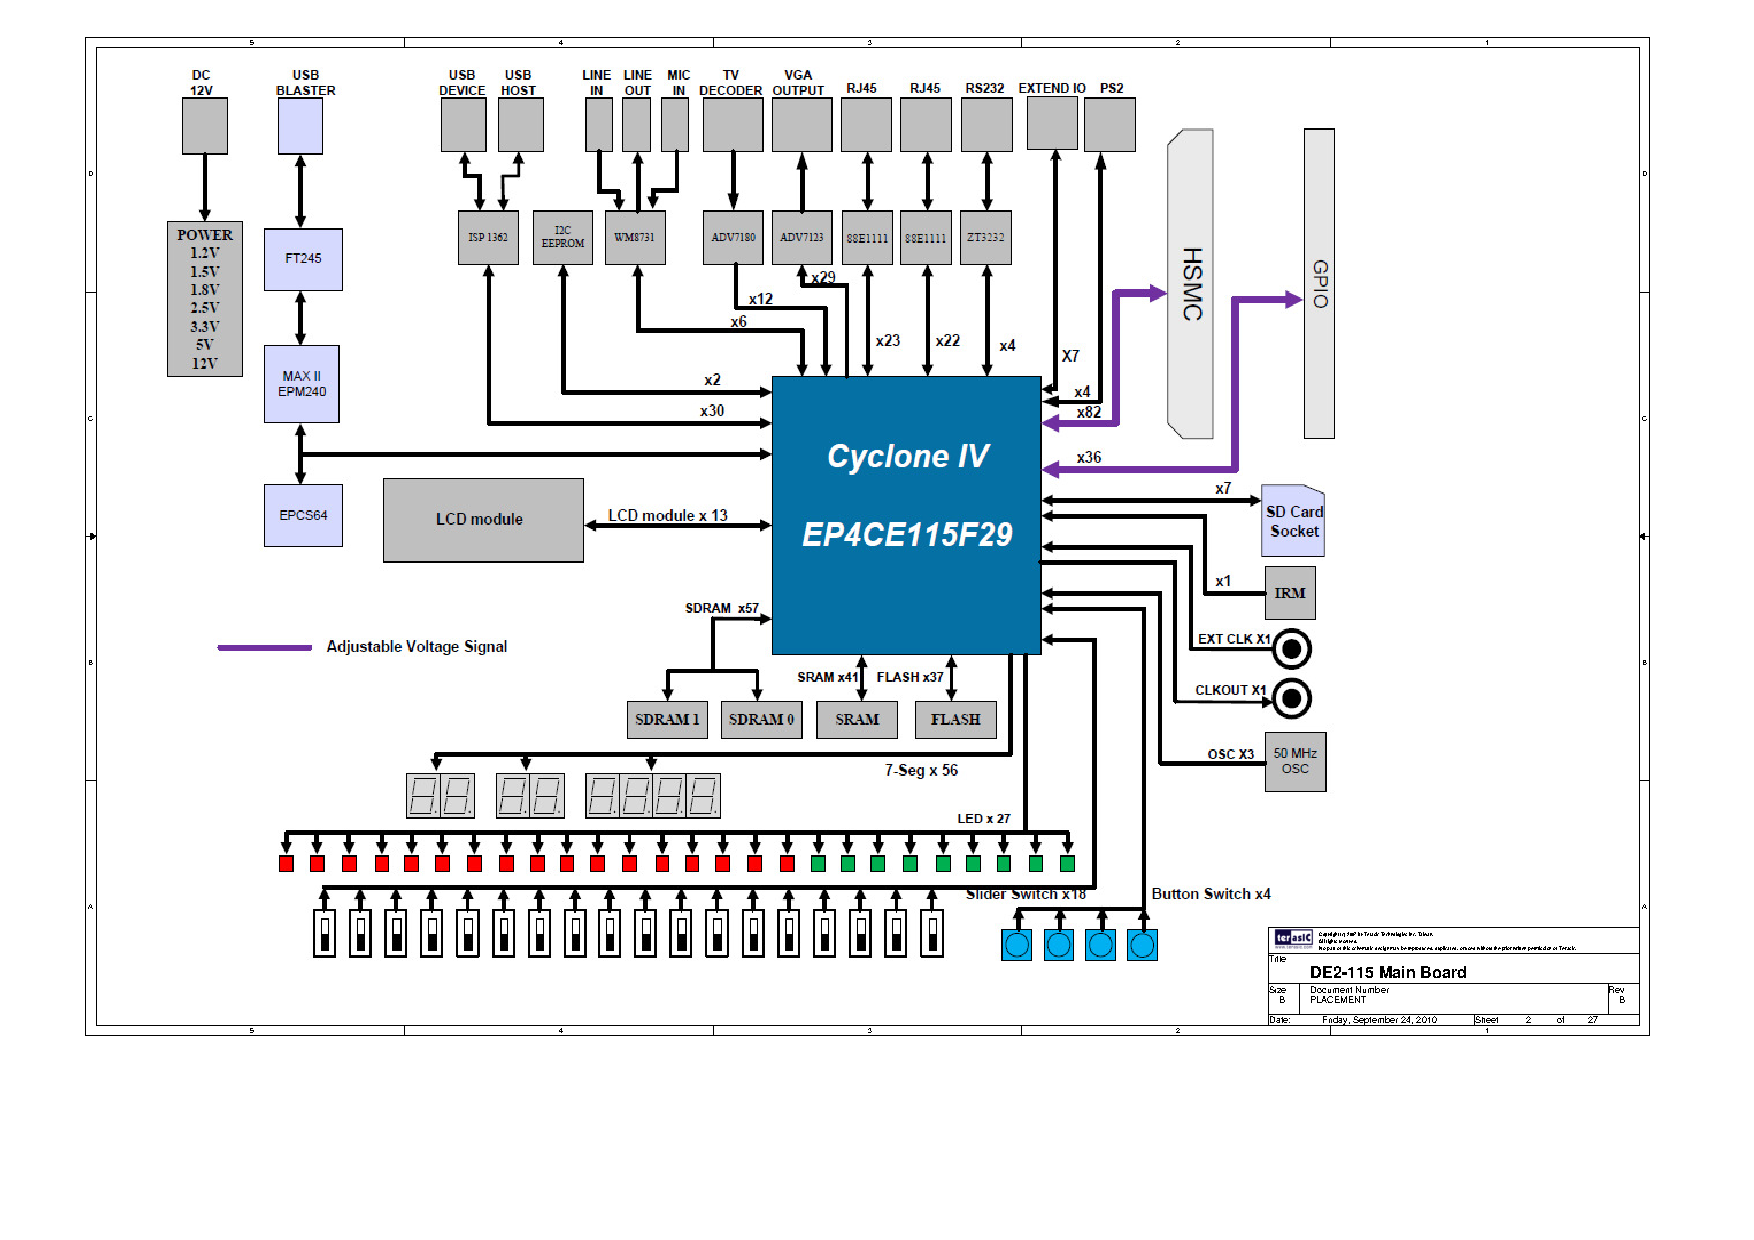
\includepdf[
 pages={-},
 nup=1x1,
 landscape=true,
 %fitpaper=true,
 %noautoscale=false,
 turn=false,
 scale=0.9, 
 %trim= 0mm 0mm 0mm 0mm,
 clip=true,
 pagecommand={},
 %delta=0mm 0mm
 offset=-6mm -7mm
]{Appendix4/pdf/De2-115.pdf}
%\label{appendix:3:1}

\end{appendices}

% *************************************** Index ********************************
\printthesisindex % If index is present

\end{document}
